\documentclass[12pt]{article}

\usepackage[italian]{babel}
\usepackage[utf8]{inputenc}
%\usepackage[T1]{fontenc}

\usepackage{wrapfig}
\usepackage{amsmath,amsfonts,amssymb,amsthm}
\usepackage{caption}
\usepackage{subcaption}
\usepackage[usenames]{color}
\usepackage{enumerate}
\usepackage{fancyhdr}
\usepackage{fancyvrb}
\usepackage{mathtools}
\DeclarePairedDelimiter{\ceil}{\lceil}{\rceil}
\usepackage{indentfirst}
\usepackage{listings}
\usepackage{paralist}
\usepackage{marvosym}
\usepackage{multicol}
\usepackage{sectsty}
\usepackage{tocloft}
% \usepackage{subfig}
\usepackage[table]{xcolor}
\usepackage{url}
\usepackage{hyperref}
\usepackage[export]{adjustbox}
\usepackage[bottom]{footmisc}
\usepackage{geometry}
\geometry{a4paper}
\usepackage{graphicx}
\usepackage{float}
\usepackage{gensymb}
\usepackage{calc}

\linespread{1.2}
\setlength{\parindent}{0pt}

\hypersetup{
    colorlinks=true,
    linkcolor=blue,
    filecolor=magenta,      
    urlcolor=blue,
    citecolor=red
}

\begin{document}

%----------------------------------------------------------------------------------------
%	TITOLO
%----------------------------------------------------------------------------------------

\begin{titlepage}

\newcommand{\HRule}{\rule{\linewidth}{0.5mm}}

\center

\textsc{\Large Relazione del progetto per il corso di \\ Sistemi Intelligenti Robotici}\\[0.5cm]

\HRule \\[0.4cm]
{\huge \bfseries Riproduzione di un \\[0.1cm] Distributed Adaptive Controller \\[0.1cm] per Agenti Robotici: \\[0.1cm] Apprendimento autonomo \\[0.5cm] della Obstacle-Avoidance}\\[0.4cm]
\HRule \\[1.cm]

\emph{A.A.2017/2018}

\vfill

\emph{Matteo Gabellini, Alessandro Cevoli}\\[3cm]

\end{titlepage}

%----------------------------------------------------------------------------------------
%	INDICE
%----------------------------------------------------------------------------------------

\tableofcontents

\section{Introduzione}

L'obiettivo di questo breve progetto è quello di riprodurre un \textbf{Distributed Adaptive Controller} per Agenti Robotici, descritto in \cite{pfeifer2001understanding} e \cite{verschure1992distributed}, che permetta di \textit{apprendere in maniera completamente autonoma e non supervisionata} il comportamento della Obstacle-Avoidance, sfruttando una semplice Artificial Neural Network di tipo Feed-Forward.

Nella fattispecie si vuole studiare come il modello di controller riprodotto è influenzato dalla presenza di un numero variabile di sensori e dalla loro posizione. Nel corso della relazione verranno descritti 3 modelli di agente robotico, ognuno dei quali si distingue per una diversa configurazione neurale.

Gli agenti robotici adoperati nel corso dell'esperimento sono totalmente simulati e sono stati realizzati tramite l'ausilio dell'ambiente virtuale di Webots (R2019a revision 1) \cite{michel2004cyberbotics}.

Nella sezione iniziale verrà illustrata brevemente la struttura dei robot adoperati sia dal punto di vista della loro morfologia e dei sensori equipaggiati che da quello della struttura della rete neurale che ne costituisce il controller. 
Nella seconda parte verranno disposte le basi implementative che hanno permesso la realizzazione dei controller.
Infine si procederà alla descrizione dei metodi di addestramento e test adoperati, quali dati sono stati raccolti in tali fasi e gli indicatori sfruttati per valutare le performance dei robot virtuali.




\section{Progettazione}

\subsection{Embodiment}

Per la realizzazione del modello del robot ci si è basati su quella di \href{https://www.cyberbotics.com/e-puck}{E-puck v2}, a cui vi sono stati aggiunti una serie di sensori extra (\textit{Bumpers}) al fine di mantenere il modello coerente a quello descritto in \cite{pfeifer2001understanding} e che fosse un buon compromesso rispetto a quello descritto in \cite{verschure1992distributed}.

\subsubsection{Sensori}

Ci limiteremo a descrivere i sensori utilizzati nella nostra versione di E-puck e utili ai fini dell'esperimento. Per la precisione verranno specificate le caratteristiche in termini di range, rumore e mapping definiti tramite le Look-Up Table che governano il comportamento di tali sensori.

\begin{itemize}
    \item \texttt{IR Distance Sensor}: Tali sensori sono queli di default presenti in E-puck. Nel nostro caso specifico sono stati programmati per ottenere una risoluzione minima di \texttt{0cm} e massima di \texttt{10cm}, con un rumore variabile tra \texttt{[0.01, 0.05]}. Per restare allineati con i valori sia del paper \cite{verschure1992distributed} che del libro \cite{pfeifer2001understanding}, si è deciso di mappare i valori simulati percepiti dal sensore in un intorno compreso tra \texttt{[0.0, 1.0]}.
    
    \item \texttt{Bumper Sensor}: Tali sensori sono stati aggiunti al modello base di E-puck al fine di modellare lo Stimolo non-Condizionato (US \cite{verschure1992distributed}) che porta l'agente a modificare la velocità delle proprie ruote e dunque spostarsi dall'ostacolo (UR \cite{verschure1992distributed}).
    Come per il sensore precedente, per restare allineati ai documenti di riferimento, la Look-Up Table è stata così definita: il sensore produce valori \texttt{\{0.0, 1.0\}} a seconda che sia avvenuta o meno una collisione, con un rumore pari a \texttt{0.01}\footnote{Ma non dovrebbe fare molta differenza porlo anche a 0.0 visto che il sensore è binario.}. I valori del sensore sono poi mappati in maniera identica in \texttt{\{0, 1\}}.
\end{itemize}

\newpage

\subsubsection{Effettori}

Gli unici effettori di cui è provvisto il nostro modello di E-puck sono i \texttt{Rotational Motor} che permettono di modulare la potenza e direzione della rotazione di una singola ruota. Dal momento che l'agente è provvisto di 2 sole ruote (una per ogni lato), sono anche presenti 2 \texttt{Rotational Motor}. Tali motori producono una velocità lineare per ogni ruota compresa tra \texttt{[0.0, 7.536]cm/sec}.

\subsubsection{Morfologia}

\begin{figure}[H]
    \centering
    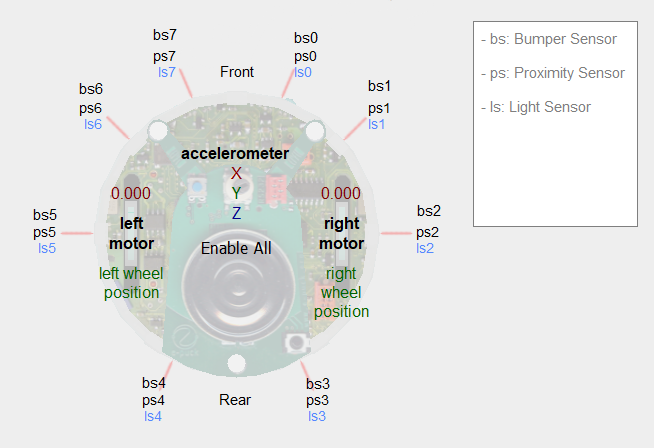
\includegraphics[scale=0.9]{figures/epuck_morphology.png}
    \caption{La morfologia del robot è quella classica del modello E-puck. I bumpers sono stati posizionati in corrispondenza di ogni \texttt{Distance Sensor} (in figura \texttt{ps}), ma in modo tale da non ostruire il raggio d'azione del sensore. Nello specifico sono posizionati attorno alla circonferenza del cilindro che costituisce il corpo principale alle senguenti angolature (leggendo in senso orario, da \texttt{bs0} a \texttt{bs7}): \texttt{1.27rad}, \texttt{0.77rad}, \texttt{0.0rad}, \texttt{5.21rad}, \texttt{4.21rad}, \texttt{3.14159rad}, \texttt{2.37rad}, \texttt{1.87rad}.}
    \label{fig:Morphology}
\end{figure}

\newpage

\subsection{Neural Network Controller}\label{lab:ANN}

Dal momento che le descrizioni dell'esperimento nei documenti di riferimento \cite{pfeifer2001understanding, verschure1992distributed} non sono totalmente coerenti dal punto di vista della descrizione del controller e della morfologia del robot utilizzato, si è deciso di realizzare più versioni del controller (\textit{senza modificarne la morfologia}). Ogni versione sfrutta o aggrega solo una parte dei sensori equipaggiati.

\paragraph{Differenze nei modelli di riferimento}
All'interno di \cite{pfeifer2001understanding} viene modellato un robot che possiede 6 sensori di prossimità affiancati ognuno da un sensore di collisione. Tali sensori sono montati lungo la metà anteriore del robot. I sensori di prossimità sono collegati ad un primo layer di 6 neuroni, i quali utilizzano una Sigmoide come funzione di attivazione. Tale layer di neuroni è a sua volta \textit{Fully Connected} con pesi variabili ad un secondo layer di input composto da ulteriori 6 neuroni. Ognuno di questi ultimi riceve in input anche il segnale proveniente da uno dei sensori di collisione. Nel secondo layer la funzione di attivazione utilizzata è la \textit{Binary Threshold}. L'incognita del modello esposto dal libro sono le connessioni del Layer di Collisione con i neuroni del layer successivo, il Motor Layer, che ne implementa i riflessi: ogni neurone del Layer di Collisione è collegato a gruppi di due ai 3 neuroni del Motor Layer. I riflessi inoltre non sono delineati all'interno della descrizione fornita e non è specificato quali azioni applicano sui motori. 


All'interno di \cite{verschure1992distributed} è presentato un controller che implementa \textit{Obstacle-Avoidance} e \textit{Fototassi}. Proseguiamo la spiegazione concentrandoci solo sulla componente di \textit{Obstacle-Avoidance}. 
Il modello proposto dal paper è provvisto di 6 sensori di prossimità, posizionati nella parte anteriore dell'agente tra $[90\degree,-90\degree]$, e 2 sensori di collisione che rivestono i due quarti anteriori del veicolo tra $[90\degree,-90\degree]$. Non è specificato il numero di ruote di cui è provvisto il robot.
In tale documento, inoltre, non si fa specificatamente riferimento all'uso di una rete neurale, bensì si parla genericamente di "\textit{learning mechanisms}" e "\textit{neural fields}", richiamandosi per la maggior parte al \textit{Classical Conditioning} e i \textit{Value System}. Nel paper l'apprendimento è infatti identificato come l'associazione di una serie di \textit{stimuli} ad una specifica \textit{response}. 

Nello specifico vengono delineati:

\begin{itemize}
    \item \textit{Conditioned-Stimuli}, associabili ai segnali percepiti dall'agente tramite i sensori di prossimità. Tali \textit{stimuli} sono organizzati in \textit{Conditioned-Stimuli Fields}. Questo "layer" modula il segnale degli \textit{stimuli} utilizzando una funzione esponenziale inversa come una funzione di attivazione.
    
    \item \textit{Unconditioned-Stimuli$^-$}, associabili ai segnali percepiti dall'agente tramite i sensori di collisione. In questo caso gli \textit{stimuli} sono organizzate in \textit{Unconditioned-Stimuli Fields$^-$}. Tali \textit{stimuli} sono collegati agli elementi dei \textit{Conditioned-Stimuli Fields} da una serie di connessioni (variabili) che vanno da quest'ultimo verso il primo.
    
    \item \textit{Unconditioned-Response}, associabili ai segnali da inviare ai motori al fine di ottenere un certo comportamento. Tali \textit{response} sono organizzati in \textit{Unconditioned-Response Fields} e ad ognuna è associato ad un "\textit{command neuron}" che ne codifica la precisa risposta ai motori (un riflesso). Tali \textit{response} sono delineate nel paper come \texttt{Advance}, \texttt{Reverse}, \texttt{TurnLeft(x degrees)} e \texttt{TurnRight(x degrees)} ma senza approfondire ne la loro implementazione, ne la loro interazione o eventuale mutua esclusione.
    
    Ogni \textit{command neuron} è collegato agli elementi dei \textit{Unconditioned-Stimuli Fields$^-$} tramite una serie di connessioni pesate e fisse che vanno da quest'ultimo verso il primo.
\end{itemize}  

Di conseguenza abbiamo deciso di semplificare il modello ponendo solo 2 neuroni nel Motor Layer che singolarmente pilotano ciascuno la propria ruota e un solo neurone nel Reverse Layer che agisce sull'output dei neuroni del motor layer modificandone il segno.
Il comportamento della sterzata risulterà emergente dalle differenti velocità "erogate" ai due motori.
Questa idea è nata seguendo l'esempio dei \textit{Braitenberg Vehicles}.

Questo tipo di modellazione inoltre riduce il problema della \textit{Behaviour Segmentation} ed una gestione altrimenti macchinosa dell'interazione tra i riflessi.

\subsubsection{Struttura generale}

\begin{figure}[H]
    \centering
    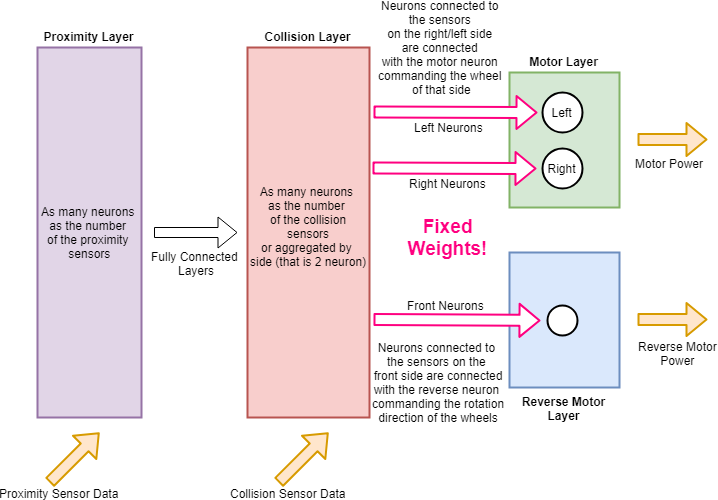
\includegraphics[scale=0.6]{figures/dac_ann_structure_generic.png}
    \caption{In figura è presentata la struttura della rete neurale, ad alto livello e generalizzata, adoperata per implementare il controller.\\ 
    Il numero dei neuroni nei layer di input dipenderà dalla configurazione dei sensori o dalle possibili astrazioni applicate su di essi. L'apprendimento inoltre avviene solo sulle connessioni presenti tra il layer di prossimità e quello di collisione.\\ 
    Tutte le altre connessioni sono fisse e poste a \texttt{1.0}. 
    Il numero di neuroni nel layer di output, invece, dipende dal numero di riflessi che si vogliono implementare nel robot. 
    Nel nostro caso l'agente deve solo eseguire l'\texttt{Obstacle-Avoidance}, di conseguenza si è posto un solo neurone per ruota che ne pilota la potenza del motore associato e un solo neurone che inverte il senso di rotazione di una di esse, necessario se il robot vuole evitare scontri frontali (inversione di marcia), per un totale quindi di 3 neuroni.}
    \label{fig:AnnStructure}
\end{figure}

\newpage

Partendo quindi dalle due strutture di riferimento sono quindi state realizzate 3 versioni del controller, tutte caratterizzate da una configurazione neurale peculiare.\label{marker:dacmodels} 
\begin{enumerate}
    \item La prima versione, visibile in figura \ref{fig:dacv2} e denominata \texttt{dacv2}, sfrutta tutti i sensori di prossimità e bumper presenti. Gli output dei sensori di prossimità sono collegati come input ai neuroni del \textit{proximity layer}. Quest'ultimi sono poi fully connected con pesi variabili ai neuroni del \textit{collision layer}, in cui ad ogni neurone di tale livello è associato un bumper. Successivamente i neuroni collegati ai bumper del lato sinistro dell'agente sono collegati ad un neurone che mappa gli input nella relativa risposta al motore che pilota la ruota sinistra. Rispettivamente i neuroni di collisione relativi al lato destro sono collegati ad un neurone che modella la risposta al motore del lato destro. Per quanto riguarda i neuroni a cui sono collegati i bumper frontali (\textit{bs0 e bs7}), essi sono anche collegati ad un neurone dedito all'attivazione del riflesso di inversione del motore. Tutti i collegamenti dal layer di collisione a quello della gestione delle risposte dei motori presentano pesi fissi.
    
    \item Nella successiva versione, denominata \texttt{dacv3} si è cercato di fornire un'implementazione simile a quella riportata nel paper \cite{verschure1992distributed}.
    In esso si ha che il robot possiede solamente 2 sensori di collisione frontali, i quali coprono rispettivamente metà della parte anteriore del robot (1/4 della circonferenza del robot). All'interno del simulatore utilizzato non vi è la possibilità di utilizzare bumper di tali dimensioni, per cui si è pensato di utilizzare gli stessi bumper della versione \textit{dacv2} e modellare i bumper descritti nel paper sfruttando la somma logica dei segnali provenienti dai bumper che coprono la relativa posizione di quelli del paper. Tale somma logica verrà poi utilizzata all'interno della funzione di composizione dei neuroni del livello di collisione.
    Come descritto in figura \ref{fig:Dacv3} si avrà quindi che per quanto riguarda la gestione del layer di prossimità è stata utilizzata la stessa configurazione della versione \textit{dacv2}. Questo layer è fully connected a 3 neuroni nel livello di collisione ai quali sono collegati rispettivamente i bumper [\textit{bs0,bs1,bs2}] (la cui somma logica modella il bumper del paper montato sulla parte destra), [\textit{bs3 e bs4}] e [\textit{bs5,bs6,bs7}] (la cui somma logica modella il bumper del papar montato a sinistra). Successivamente il neurone che si occupa di rilevare le collissioni a destra è collegato al neurone che mappa la risposta del motore destro e viceversa per quanto riguarda i neuroni del livello di collisione e dei motori della parte sinistra. Entrambe le uscite dei neuroni di destra e sinistra del livello di collisione sono collegate al neurone che gestisce il riflesso di reverse. Per quanto riguarda il neurone del livello di collisione centrale (\ref{fig:Dacv3}) quello che riceve gli input dai bumpers \textit{bs3 e bs4} esso al momento non è collegato a nessun neurone del layer motori. Esso è stato comunque lasciato in quanto in futuro potrebbe essere utilizzato per implementare la gestione del riflesso "advance" citato nel paper, che al fine della collision-avoidance non è risultato necessario.
    
    \item Partendo dall'implementazione della versione \textit{dacv2} si è realizzata un'ultima versione, denominata \texttt{dacv4}(visibile in figura \ref{fig:dacv4}),  in cui i sensori di prossimità posteriori \texttt{\{ps3, ps4\}} e i relativi bumpers \texttt{\{bs3, bs4\}} sono scollegati dal controller. Ergo, vengono adoperati ai fini dell'apprendimento esclusivamente i sensori di prossimità e bumper frontali e laterali. Tale implementazione è nata dalla necessità di capire se l'uso dei sensori posteriori influisse negativamente sull'apprendimento generale del robot.
    
\end{enumerate}

\begin{figure}[H]
    \centering
    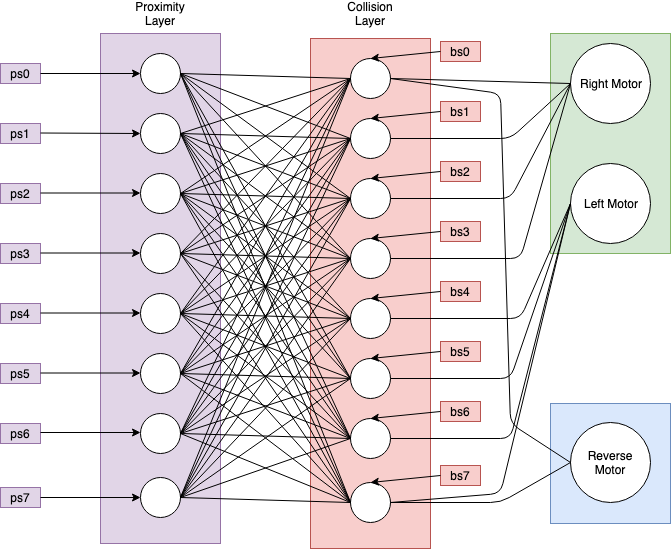
\includegraphics[scale=0.45]{figures/NetVersion2.png}
    \caption{Schema della rete \texttt{dacv2}}
    \label{fig:dacv2}
\end{figure}

\begin{figure}[H]
    \centering
    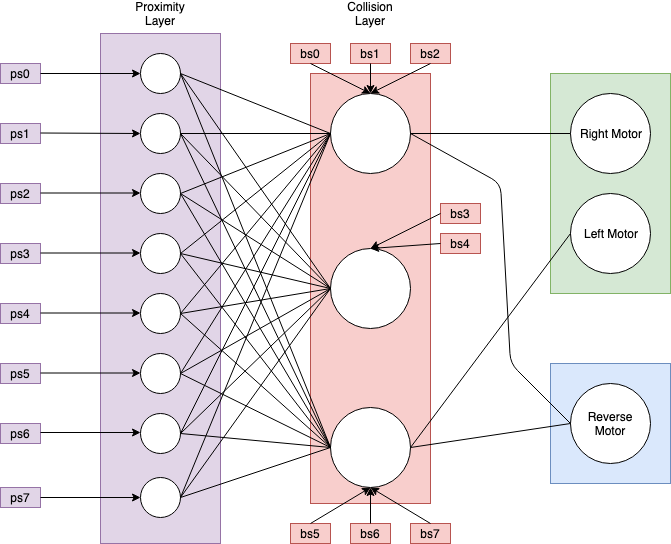
\includegraphics[scale=0.45]{figures/NetVersion3.png}
    \caption{Schema della rete \texttt{dacv3}}
    \label{fig:Dacv3}
\end{figure}

\begin{figure}[H]
    \centering
    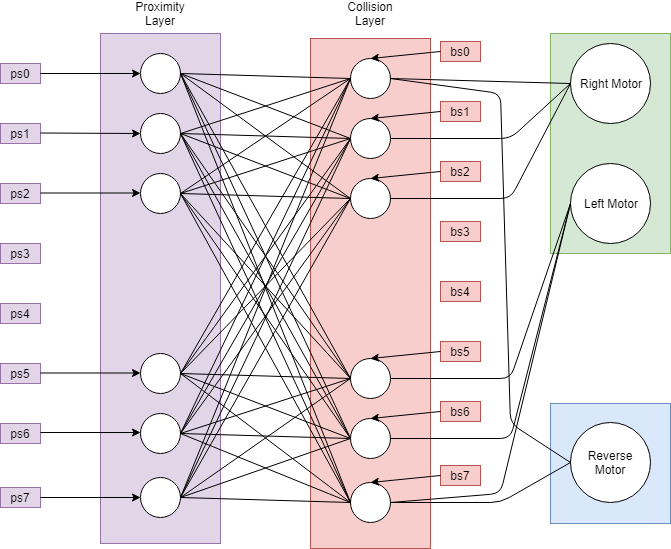
\includegraphics[scale=0.45]{figures/NetVersion4.png}
    \caption{Schema della rete \texttt{dacv4}}
    \label{fig:dacv4}
\end{figure}

In tutte e tre le versioni il layer di "reverse" contiene un solo neurone che si deve attivare qualora tutti i neuroni del layer di collisione associati con i bumper frontali risultano attivi. Il verso della marcia dipenderà dall'eventuale numero degli altri neuroni attivi nel layer di collisione e a quale lato (sinistro o destro) questi fanno parte. Il lato che possiede meno neuroni attivi assume marcia negativa. In caso di parità sarà sempre il motore di destra ad assumere senso negativo.

% \newpage

\subsubsection{Input Composition, Activation  Functions e Output Functions}

Prima di esporre le varie formule vogliamo fare dei chiarimenti sulla notazione usata, nello specifico negli indici, al fine di evitare confusione e velocizzare la compresione di ciò che viene riportato.

\begin{itemize}
    \item Indice ${i}$ indica sempre una entità del Layer precedente
    \item Indice ${k}$ indica sempre una entità proveniente dai sensori, usualmente $k==j$
    \item Indice ${j}$ indica sempre una entità del layer attuale
    \item $w_{ij}$ è il peso della connessione tra il neurone $i$ del livello precedente ed il neurone $j$ del layer successivo
    \item $N_j$ è l'insieme di neuroni del layer precedente connessi al neurone $j$ del layer successivo
    \item $o_j$ è l'output del neurone $j$ del layer corrente
    \item $o_i$ è l'output del neurone $i \in N_j$ appartenente al layer precedente
\end{itemize}

\newpage

\textbf{Proximity} = $
    \begin{cases}
        h_j=p_k & \text{where $p_k$ is the output of sensor $ps_k$} \\
        a_j=e^{-h_j} & \\
        o_j=a_j & \\
    \end{cases}
$\\

\hfill\break

\textbf{Collision} = $
    \begin{cases}
        h_j = c_k + \sum_{i\in N_j} w_{ij}\cdot o_i \\
        a_j = \begin{cases}
           1 & \text{if $h_j \ge \tau_{Collision}$,}\\
           0 & \text{else.}
        \end{cases} & \\
        o_j = a_j & \\
    \end{cases}
$\\

\hfill\break
Where $c_k$ is the output of sensor $bs_k$ in net versions \texttt{dacv2} and \texttt{dacv4} while is the logic sum of outputs of $bs$ sensors connected to the neuron in net version \texttt{dacv3}. 

\hfill\break

\textbf{Reverse} = $
    \begin{cases}
        h_j = \sum_{i\in N_j} w_{ij}\cdot o_i & \\
        a_j = \begin{cases}
           1 & \text{if $h_j \ge \tau_{Reverse}$,}\\
           0 & \text{else.}
        \end{cases} & \\
        o_j = a_j & \\
    \end{cases}
$\\

\hfill\break

\textbf{Motor} = $
    \begin{cases}
        h_j = \sum_{i\in N_j} w_{ij}\cdot o_i & \\
        a_j = \begin{cases}
           h_j & \text{if $h_j \ge \tau_{Motor}$,}\\
           0 & \text{else.}
        \end{cases} & \\
        o_j = a_j \cdot \texttt{MIN\_V} & \text{where \texttt{MIN\_V} is a bounding constant} \\
    \end{cases}
$\\

\hfill\break

La funzione di attivazione nel Motor Layer potrebbe tranquillamente essere una funzione linerare tale che $a_j=h_j$. Il comportamento risultante è il medesimo.

\newpage

\subsubsection{Learning Function}

La funzione di apprendimento adoperata all'interno della rete è la medesima proposta all'interno del materiale di riferimento, ovvero \textit{Hebbian Learning with Active Forgetting}.

$$\Delta{w_{ij}}=\frac{\eta \cdot o_i \cdot o_j - \epsilon \cdot w_{ij} \cdot \overline{\rm o}_{Collision}}{|Proximity|}$$
\hfill\break
Questo permette all'agente di apprendere in maniera continua ma limitata ai soli "eventi di collisione", o più precisamente solo quando nel layer di collisione sono presenti dei neuroni attivi (il quale non implica necessariamente una collisione in realtà).

\section{Implementazione}

Esponiamo ora alcuni dettagli implementativi relativi alla struttura delle reti e alla loro logica evolutiva. 

%implementazione della struttura
\begin{itemize}
    \item Per quanto riguarda l'implementazione della \textit{struttura della rete neurale} per modellare l'uscita corrente dei neuroni di un layer si è deciso di ricorrere a dei dizionari: la chiave rappresenta l'id del neurone e l'elemento relativo è il valore di uscita corrente del neurone.
    I vari dizionari che rappresentano i layer costituiscono poi gli elementi di un ulteriore dizionario dove la chiave è l'id del layer.
    
    \item Considerando che non tutte le connessioni tra i layer sono fully connected si è deciso di modellare le connessioni attraverso dei \textit{dizionari di dizionari} dove, prendendo in considerazione due layer, le chiavi del primo dizionario sono gli id dei neuroni del livello corrente ed ogni elemento corrisponde ad un un ulteriore dizionario. Per quest'ultimo le chiavi sono gli id dei neuroni del livello precedente a cui è connesso e gli elementi sono i relativi pesi.
    
    \item Relativamente alle funzioni di composizione,attivazione e uscita sono state rispettivamente implementate anch'esse con dei dizionari, dove la chiave dei dizionari costituisce l'id del layer e l'elemento è la lambda che definisce la funzione.
\end{itemize}

%spiegazione logica evolutiva
\begin{itemize}
    \item Per quanto riguarda la logica evolutiva, riportata in figura \ref{fig:evolutionLogic}, per ogni step di simulazione vengono per prima cosa campionati i valori dei sensori. Successivamente si passa ad elaborare lo stato corrente della rete, elaborando per ogni livello il valore di output di ogni neurone sfruttando le lambda function precedentemente citate. Una volta aggiornato lo stato della rete, si passa a calcolare le velocità dei motori sfruttando come input le uscite dei layer motori e di quello di reverse.
    Nel caso in cui siamo in modalità train della rete, una volta calcolata e applicata la velocità ai motori, si passa ad eseguire l'aggiornamento dei pesi tra i collegamenti del layer di prossimità e quello di collisione, sfruttando la \textit{Hebbian Learning with Active Forgetting} precedentemente citata.
\end{itemize}

\begin{figure}[H]
    \centering
    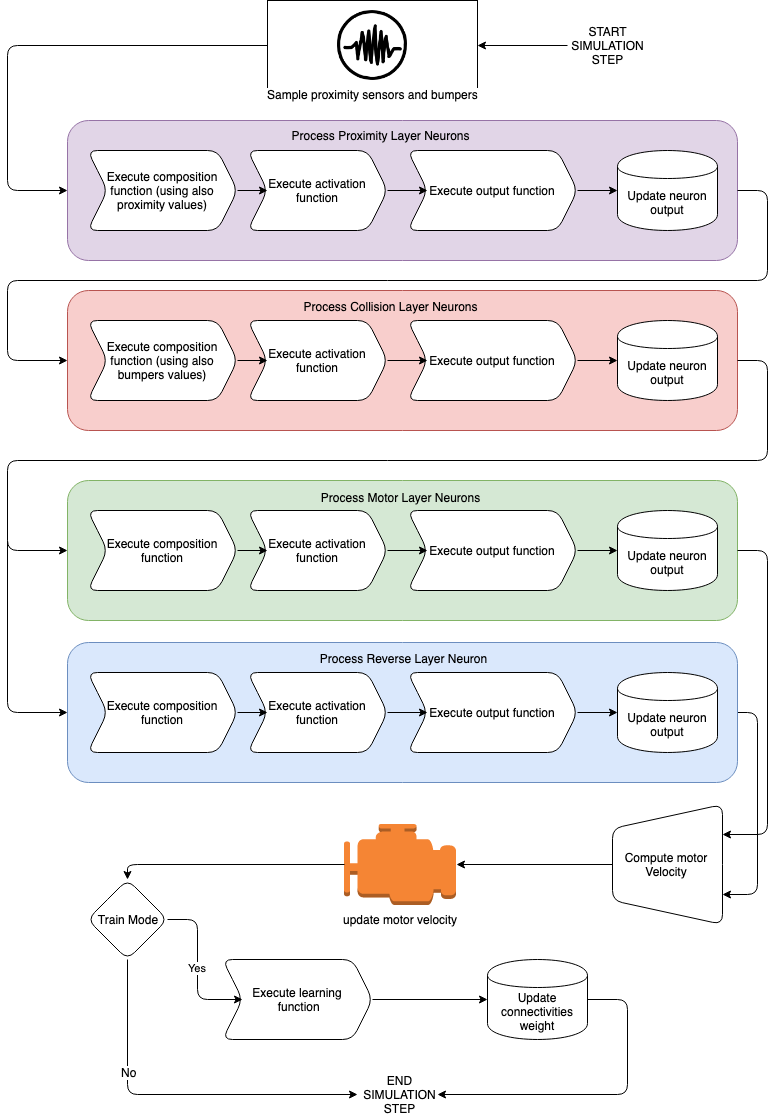
\includegraphics[scale=0.45]{figures/SimulationStep.png}
    \caption{Logica evolutiva della rete}
    \label{fig:evolutionLogic}
\end{figure}

%dettagli sull'implementazione dei riflessi dei motori
Entrando nel merito della gestione dei riflessi dei motori, come già precedentemente citato, all'interno del materiale di ricerca consultato vi erano solo indicazioni vaghe relativamente a come fossero realmente implementati. 
Perciò in questo caso abbiamo effettuato una progettazione autonoma e delle prove implementative per vedere quali fossero la strategie più adatte a gestire le nostre esigenze. Abbiamo ad esempio provato ad applicare velocità fisse, dinamiche e/o a cercare di ottenere gradi di sterzata predefiniti.
Alla fine si è deciso di prendere come valore base della velocità il valore d'uscita dei neuroni del livello motore. Ciò permette di ottenere un valore proporzionale al numero di neuroni attivi nel livello di collisione e quindi deviare maggiormente verso la direzione dove vengono rilevati meno ostacoli.

A tali velocità vengono poi applicati dei controlli:
\begin{itemize}
    \item Il primo evita che il robot rimanga fermo verificando se entrambe le velocità sono a 0. In tal caso la velocità da assegnare alle ruote viene impostata ad un valore di default predefinito.
    \item Il secondo controllo viene effettuato nel caso in cui il neurone di \textit{reverse} sia attivo. In tal caso viene controllato quale tra le due velocità è la minore e per essa viene impostato un valore negativo della velocità. Questo in caso di reverse, porterà il robot a girare su stesso verso la direzione dove vi sono meno ostacoli. Nel caso in cui le due velocità siano uguali si è scelto di sterzare sempre verso destra.
\end{itemize} 

\section{Risultati}

Come preannunciato nella sezione introduttiva, l'obiettivo principale dello studio è quello di confrontare tra loro diversi modelli di \texttt{dac}, ognuno dei quali caratterizzato da una differente modellazione della rete neurale che implementa in meccanismo di apprendimento del controller, e verificare come il meccanismo di apprendimento è influenzato dalla differente configurazione sensoriale (virtuale \ref{lab:ANN}) che li caratterizza.

I dati di seguito riportati sono relativi all'addestramento e test dei vari modelli di robot realizzati. Per ognuno di essi si sono esplorati diversi (sotto) spazi di valori dei parametri che guidano il comportamento e l'apprendimento dell'agente.

Al fine di concentrarsi ai soli parametri non banali, si è deciso di lasciare fisse le soglie di attivazione $\tau_{Motor}=1.0$ e $\tau_{Reverse}=2.0$. Queste soglie risultano banali in quanto:

\begin{itemize}
    \item Ogni neurone del layer di Collisione produce solo valori di output \texttt{\{0, 1\}}
    
    \item Si vuole modulare la velocità delle ruote in base al numero di neuroni attivi ($o_i=1.0$) su un determinato lato
    
    \item Si vuole invertire il senso di marcia se e solo se entrambi i neuroni frontali sono attivi ($o_0=1.0 \wedge o_7=1.0$)
\end{itemize}

Di conseguenza, nel caso di $\tau_{Motor}=1.0$, si ha un comportamento equivalente a $a_j = h_j$, che porta ad avere un incremento della velocità in una delle ruote proporzionale al numero di neuroni attivi collegati al neurone che soprassiede tale ruota. Nel caso di $\tau_{Reverse}$, la soglia dovrà essere $\tau_{Reverse}=N_{Reverse_j}$, nel nostro caso $N_{Reverse_j}=2.0$, se vogliamo che questi si attivi se e solo se tutti i neuroni ad esso connessi siano attivi.\\
\hfill\break
Dunque i parametri della quale si è deciso di esplorare lo spazio delle soluzioni sono:

\begin{itemize}
    \item $\eta$ -- Learning Rate
    \item $\epsilon$ -- Forget Rate
    \item $\tau_{Collision}$ -- Collision Threshold
\end{itemize}

\newpage

\subsection{Addestramento e Test}
% Elenca per ogni modello generato quali sono i range di parametri esplorati
% e perchè sono stati scelti questi parametri

Ogni modello descritto in \ref{marker:dacmodels} è stato addestrato, per ogni parametro, su un range di valori che fosse contenuto ma risultasse significativo, ovvero che contenesse con buona probabilità una o più configurazioni di parametri che avrebbero portato l'agente ad un corretto o almeno parziale apprendimento del comportamento. Questo range è stato definito in maniera totalmente empirica: prima dell'esecuzione dell'addestramento in modalità "batch" sono state avviate manualmente una serie di simulazioni di addestramento al fine di individuare un paio di esempi funzionanti, attorno alla quale è stato definito (grossolanamente) un range di valori per ogni parametro.

Sebbene in \cite{verschure1992distributed} fossero indicati alcuni di questi parametri con precisione ($\eta = 0.1, \epsilon = 0.5, \tau_{Collision} = 0.5$), test manuali effettuati con tali parametri non hanno portato risultati significativi. Ci si è dunque serviti di tali elementi solo come spunto iniziale di studio dello spazio dei parametri.

Nello specifico ogni modello ogni modello è stato addestrato con i seguenti range di parametri:

\begin{itemize}
    \item \texttt{dacv2} $\begin{cases}
            \eta \in [0.035, 0.065] & \text{with $\delta_{step}=0.005$}\\
            \epsilon \in [0.6, 0.9] & \text{with $\delta_{step}=0.05$}\\
            \tau_{Collision} \in [0.65, 0.95] & \text{with $\delta_{step}=0.05$}\\
    \end{cases}$
  
    \item \texttt{dacv3} $\begin{cases}
            \eta \in [0.065, 0.095] & \text{with $\delta_{step}=0.005$}\\
            \epsilon \in [0.6, 0.9] & \text{with $\delta_{step}=0.05$}\\
            \tau_{Collision} \in [0.55, 0.95] & \text{with $\delta_{step}=0.05$}\\
    \end{cases}$
    
    \item \texttt{dacv4} $\begin{cases}
            \eta \in [0.065, 0.1] & \text{with $\delta_{step}=0.005$}\\
            \epsilon \in [0.6, 0.9] & \text{with $\delta_{step}=0.05$}\\
            \tau_{Collision} \in [0.65, 0.95] & \text{with $\delta_{step}=0.05$}\\
    \end{cases}$
\end{itemize}
\hfill\break
% Specifica il tempo di apprendimento assegnato ad ogni agente

Sia in fase di addestramento che in fase di test si è lasciato l'agente ad apprendere o girovagare all'interno dell'arena per un tempo pari a 2h (del simulatore).

% Mostra immagine Arena Training
% Mostra immagine Arena Test
\begin{figure}[H]
    \centering
    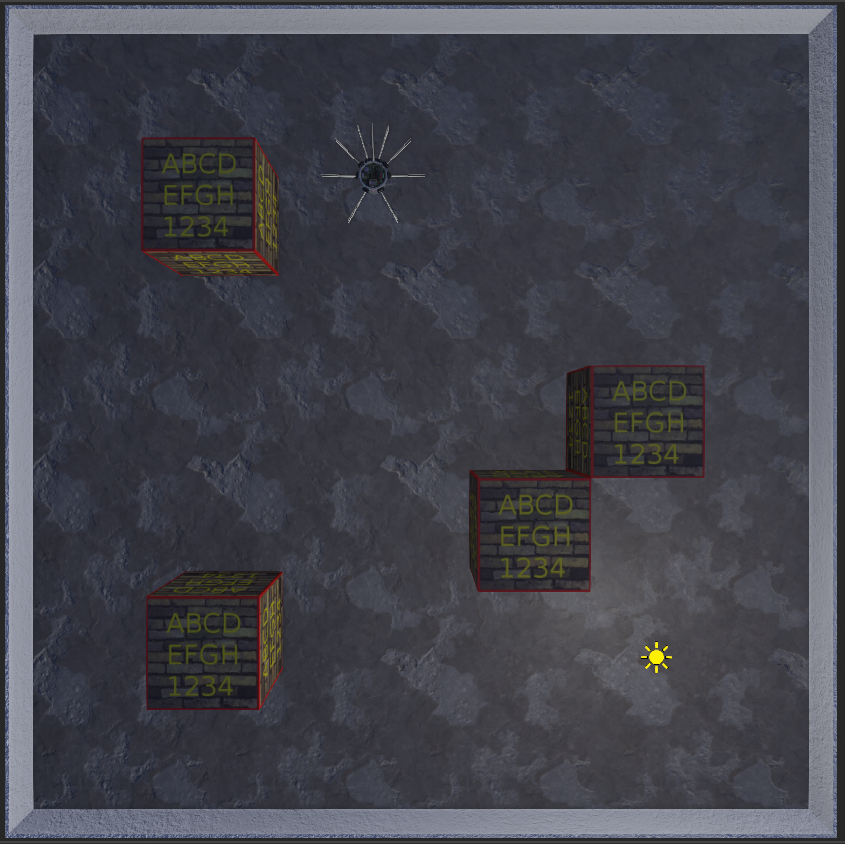
\includegraphics[scale=0.32,valign=t]{figures/train_arena.png}
    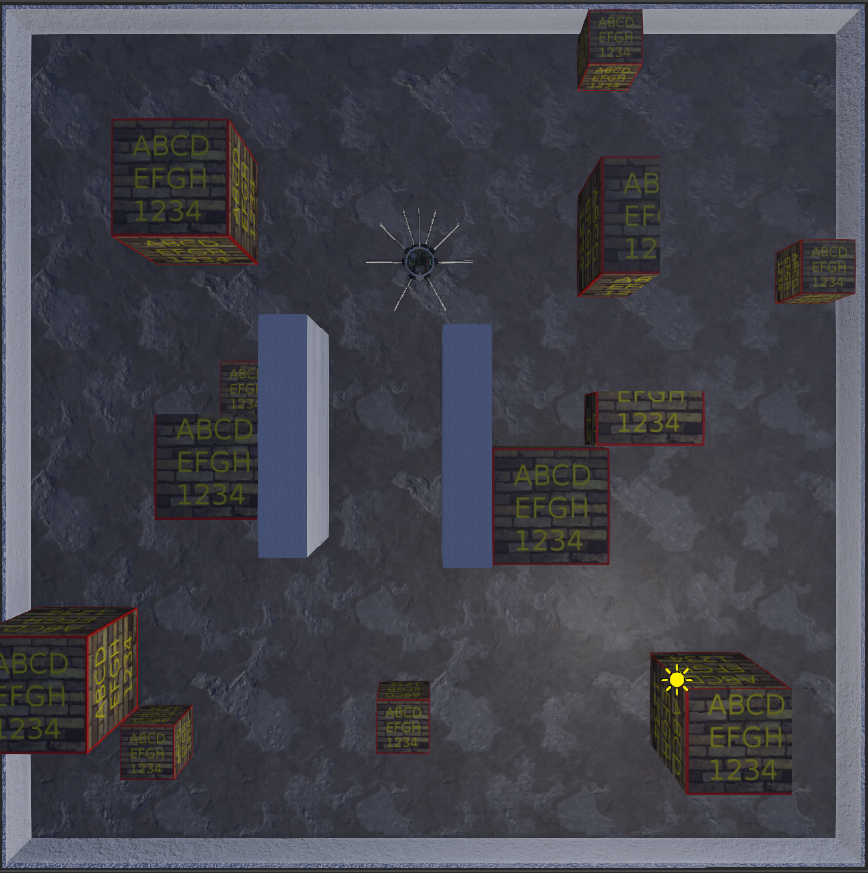
\includegraphics[scale=0.309,valign=t]{figures/test_arena.png}
    \caption{L'arena di addestramento (a sinistra) è stata realizzata volutamente semplice al fine di consentire all'agente di "apprendere" solo le situazioni di base, lasciando all'arena di test (visibile nell'immagine a destra) di verificare se il robot fosse in grado di generalizzare il comportamento appreso e in caso presentare comportamenti emergenti per configurazioni novelle degli ostacoli.}
    \label{fig:TrainArena}
\end{figure}

\subsection{Performance}

% Specifica quali dati sono stati raccolti nel corso delle simulazioni
% sia di train che di test

Nel corso di ogni simulazione sono stati raccolti, per ogni step del robot, le seguenti informazioni:

\begin{itemize}
    \item \texttt{position} -- Posizione in coordinate cartesiane
    \item \texttt{collision} -- Valore booleano che indica se uno dei bumper ha registrato una collisione
    \item \texttt{activation} -- Valore booleano che indica se vi è stata una attivazione di almeno un neurone nel Layer di Collisione.
    \item \texttt{step\_number} -- Numero del passo effettuato dal robot
\end{itemize}

Per ogni simulazione si è prodotto un log contente tali informazioni e il modello della Artificial Neural Network utilizzata o prodotta da quell'agente.

% Specifica quali indicatori e discriminatori sono stati estratti dai dati 
% e perché, delineando le caratteristiche dei falsi positivi.

Sulla base del log prodotto si è eseguita una aggregazione dei dati, individuando le seguenti caratteristiche:

\begin{itemize}
    \item \texttt{event} -- Tipo di evento. E' ricavato dall'associazione dei parametri \texttt{activation} e \texttt{collision} ed individua 4 possibili situazioni:
        \begin{itemize}
            \item \texttt{(a:False, c:False)} -- \texttt{Going by} -- l'agente non ha avuto collisioni con alcun oggetto, ne vi è stata l'attivazione di un neurone di collisione a causa di una collisione o di una schivata.
            
            \item \texttt{(a:True, c:False)} -- \texttt{Avoidance} -- Vi è stata un'attivazione nel Layer di Collisione senza che vi sia stata una vera e propria collisione. Questo significa che l'agente ha appreso un'associazione tra gli stimoli prodotti dai sensori di prossimità e quelli di collisione, portando all'attivazione del neurone prima che vi sia una effettiva collisione e inducendo dunque il robot a sterzare in \textit{qualche} direzione.
            
            \item \texttt{(a:True, c:True)} -- \texttt{Collision} -- Vi è stata una attivazione nel Layer di Collisione indotta da una collisione con un oggetto dell'arena.
            
            \item \texttt{(a:False, c:True)} -- \texttt{Error} -- Potrebbe avvenire quando vi è una collisione con un oggetto ma ciò non porta ad un'attivazione di nessun neurone all'interno del layer dedicato. Questo è solitamente sintomo di un set di parametri non idonei, come per esempio un $\tau_{Collision}$ eccessivamente alto in proporzione a $\eta$ e $\epsilon$.
        \end{itemize}
    
    Nel nostro caso i tipi di evento d'interesse sono \texttt{Avoidance} e \texttt{Collision}.
        
    \item \texttt{nCollideSteps} e \texttt{nAvoidSteps} -- Indica il numero di passi del robot associati a quel tipo di evento.
    
    \item \texttt{\%CollideSteps} e \texttt{\%AvoidSteps} -- Indicano la percentuale del tipo di eventi sul numero totale di passi che producono un'attivazione nel layer di collisione, ergo solo per eventi di tipo \texttt{Avoidance} e \texttt{Collision}. 
    
    $$\texttt{\%AvoidSteps} = \frac{\texttt{nAvoidSteps}}{\texttt{nSteps} | \texttt{activation}=True}$$
    $$\texttt{\%CollideSteps} = \frac{\texttt{nCollideSteps}}{\texttt{nSteps} | \texttt{activation}=True}$$
   
    \item \texttt{std(x)} e \texttt{std(z)} -- Indicano la deviazione standard sugli assi orizzontali \texttt{x} e \texttt{z}. Questi valori risultano particolarmente discriminanti in fase di Test per individuare \textit{Falsi Positivi}: i modelli addestrati della rete neurale che portano l'agente a girare su stesso con avanzamenti minimali ma ottengono degli score percentuali elevati. Girando su loro stessi, questi modelli tendono a non esplorare l'arena, portandoli ad ottenere una deviazione standard poco elevata.
    
    \item \texttt{nCollideEvents} e \texttt{nAvoidEvents} -- Indica il numero di eventi verificatisi. Un singolo evento è dato dall'aggregazione di "step" continui appartenenti al medesimo tipo di evento.
    
    \item \texttt{mCollideSteps} e \texttt{mAvoidSteps} -- Indica il numero medio di passi adoperato per superare un certo tipo di evento. Questo valore è significativo solo per eventi di tipo \texttt{Avoidance} e \texttt{Collision} e da una valutazione differente sulla bontà del comportamento appreso dall'agente. Sono calcolati rispettivamente come $\texttt{mCollideSteps} = \frac{\texttt{nCollideSteps}}{\texttt{nCollideEvents}}$ e $\texttt{mAvoidEvents} = \frac{\texttt{nAvoidSteps}}{\texttt{nAvoidEvents}}$.
    
\end{itemize}

I dati mostrati nei seguenti grafici sono relativi a dati già filtrati dai \textit{Falsi Positivi}. L'insieme di dati raccolti e già aggregati può essere reperito al seguente url \url{https://goo.gl/N83Uud}. 

I grafici sono da interpretarsi nel seguente modo:
\begin{itemize}
    \item Ogni colonna verticale rappresenta un modello del controller addestrato. La larghezza di ognuna di esse è inversamente proporzionale al valore di \texttt{mAvoidSteps}.
    \item Sull'asse delle ordinate sono rappresentati gli score percentuali \texttt{\%AvoidSteps}.
    \item Sull'asse delle ascisse sono rappresentate triplette ordinate del tipo $(\eta, \epsilon, \tau)$ che identificano uno specifico controller. Le "milestone" visibili sull'asse indicano il cambiamento del parametro $\eta$ e $\epsilon$. Lo spazio di valori tra ogni "milestone" presenta le combinazioni ordinate di $\tau$.
    \item Per la fase di test sono stati verificati i soli modelli che in fase di addestramento hanno ottenuto uno $\texttt{\%AvoidSteps} > 0.8$, visualizzato dalla "hotline" rossa posta in tutti i grafici. 
\end{itemize}

% Mostra i grafici risultati per ogni modello

\newpage
\thispagestyle{empty}
\newgeometry{top=5mm, bottom=10mm}

\begin{figure}[H]
    \centering
    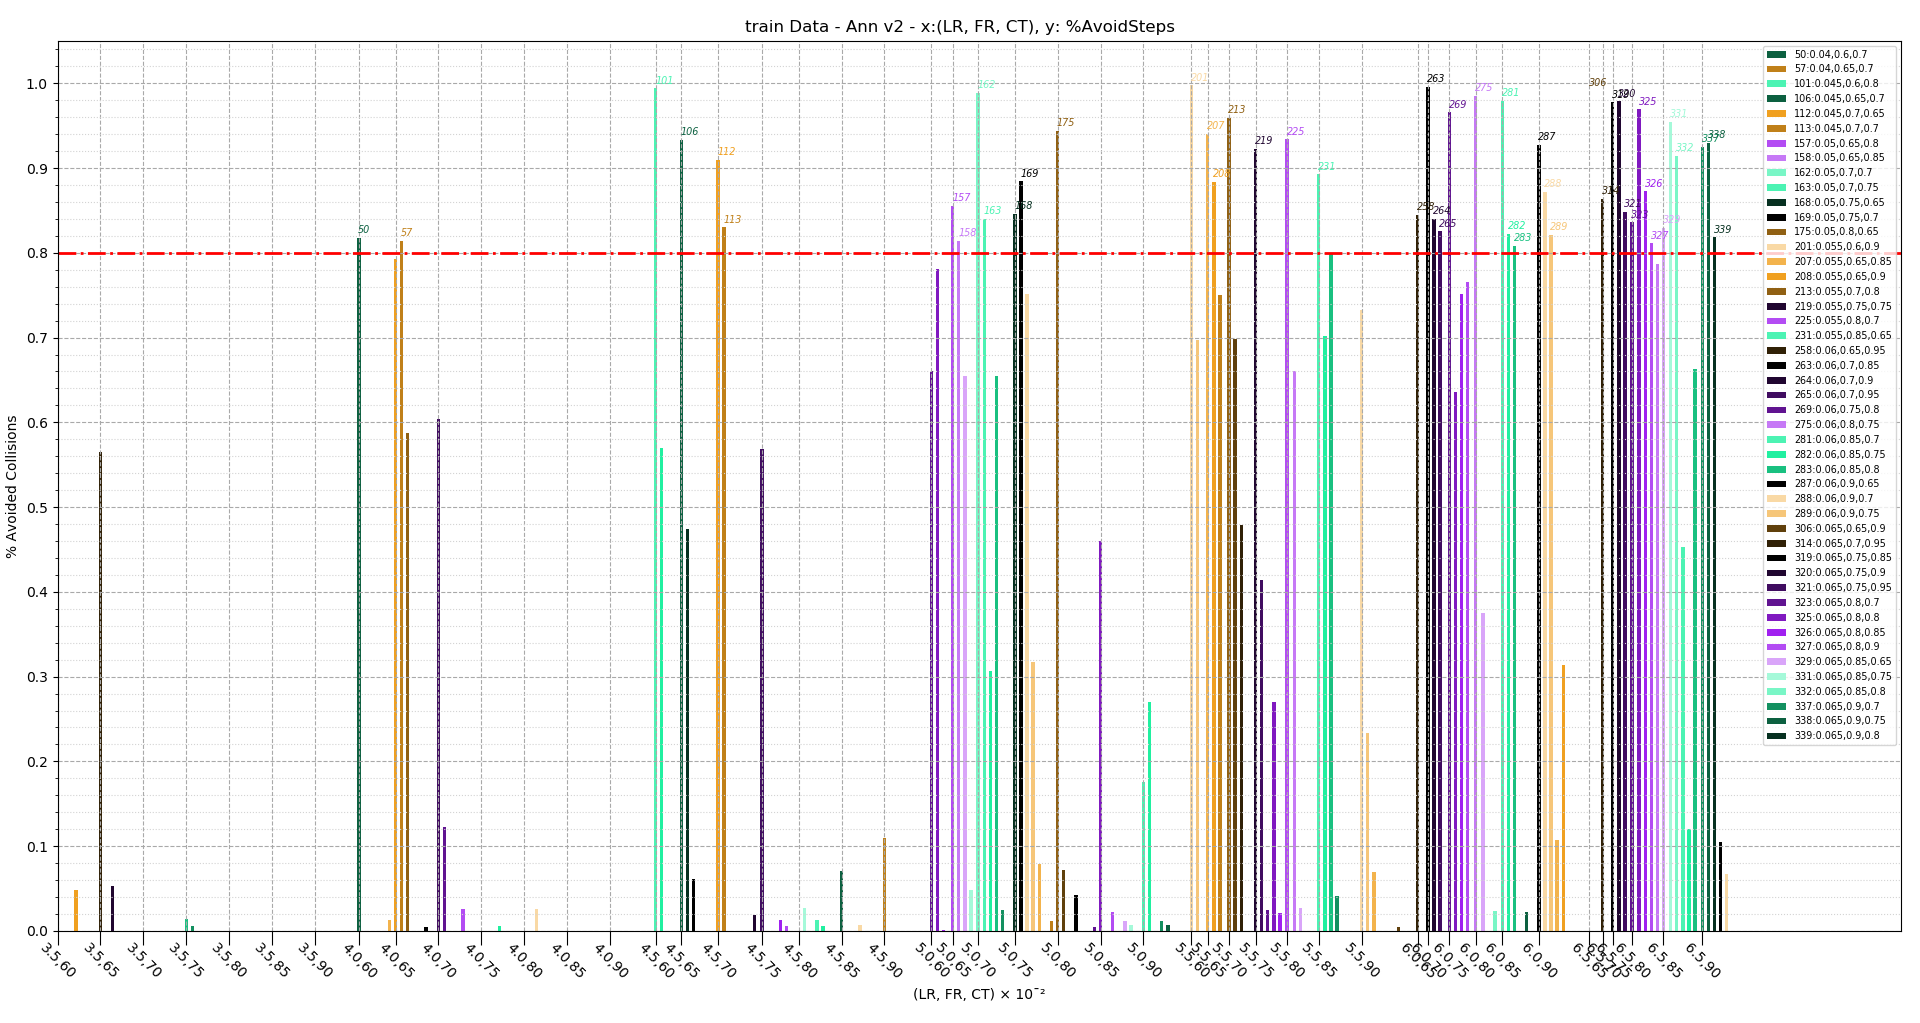
\includegraphics[scale=0.55,rotate=-90]{figures/train_annv2_2d.png}
    \caption{}
    \label{fig:TrainV2}
\end{figure}

\newpage
% \restoregeometry
\thispagestyle{empty}
% \newgeometry{top=5mm, bottom=10mm}

\begin{figure}[H]
    \centering
    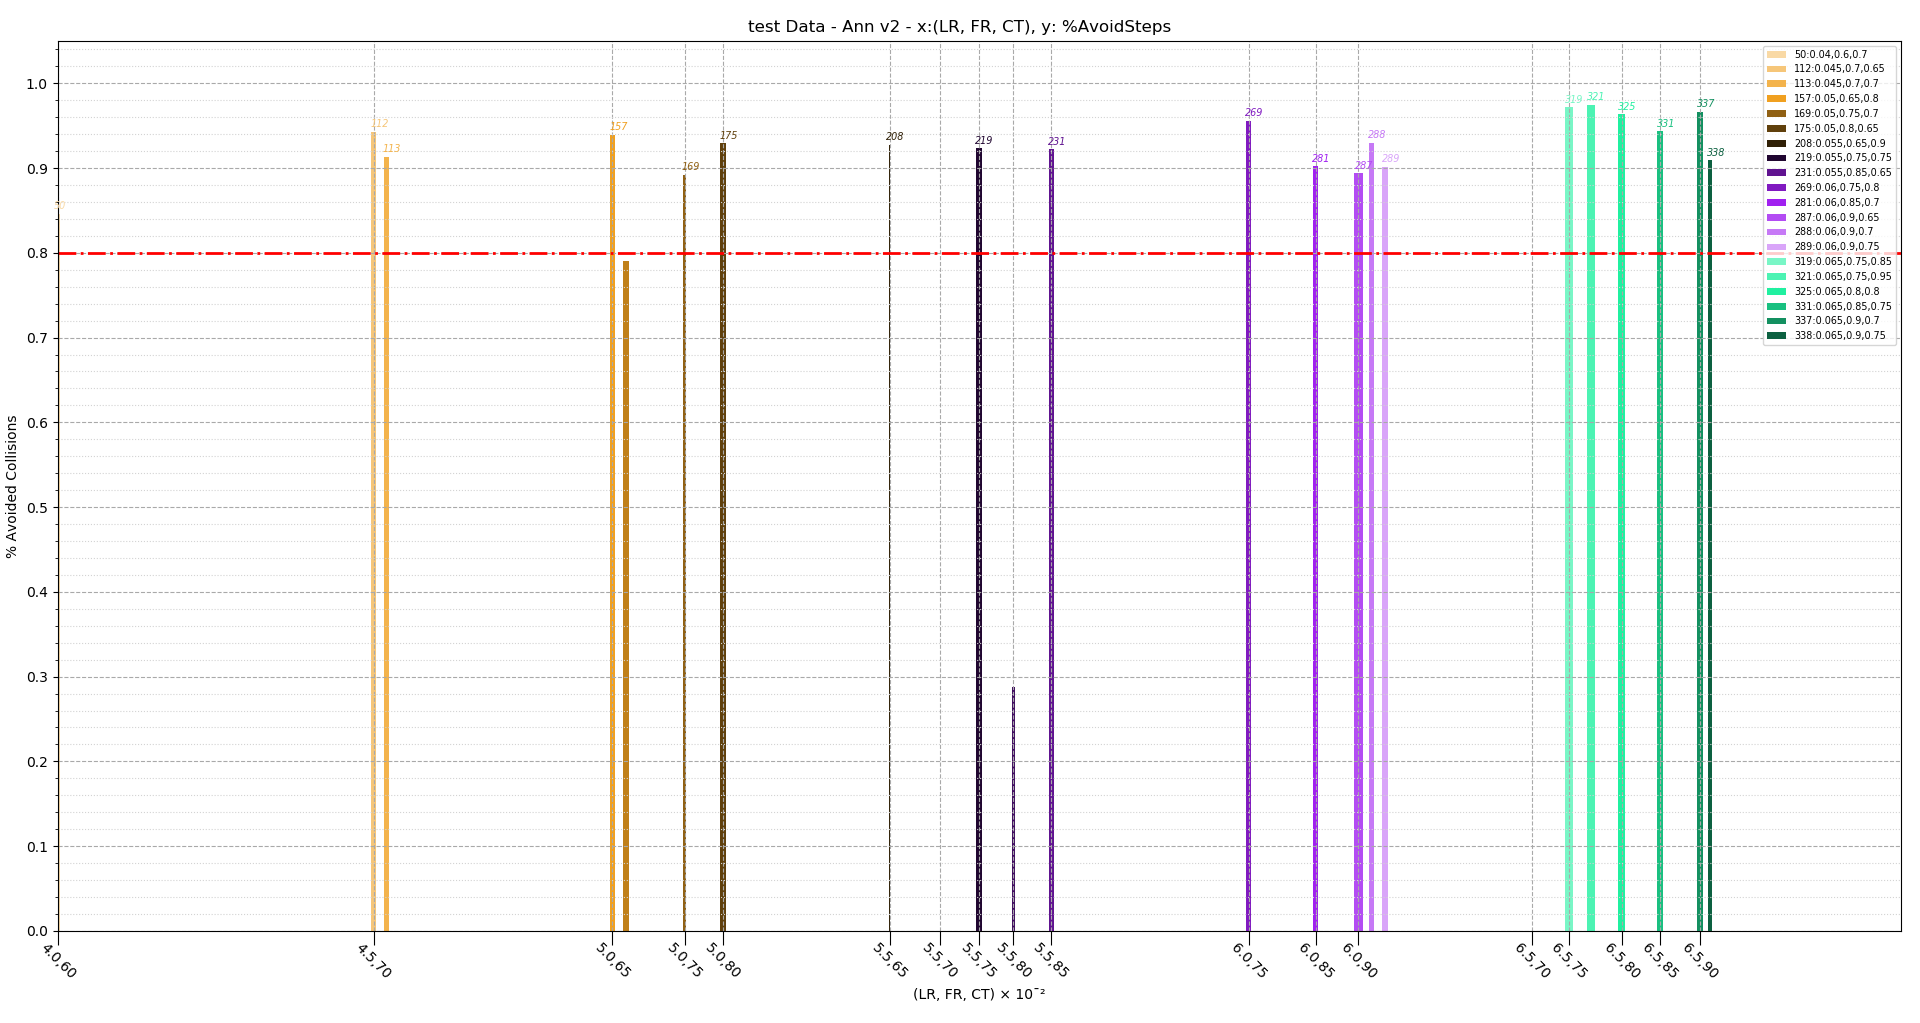
\includegraphics[scale=0.55,rotate=-90]{figures/test_annv2_2d.png}
    \caption{}
    \label{fig:TestV2}
\end{figure}

\newpage
% \restoregeometry
\thispagestyle{empty}
% \newgeometry{top=5mm, bottom=10mm}

\begin{figure}[H]
    \centering
    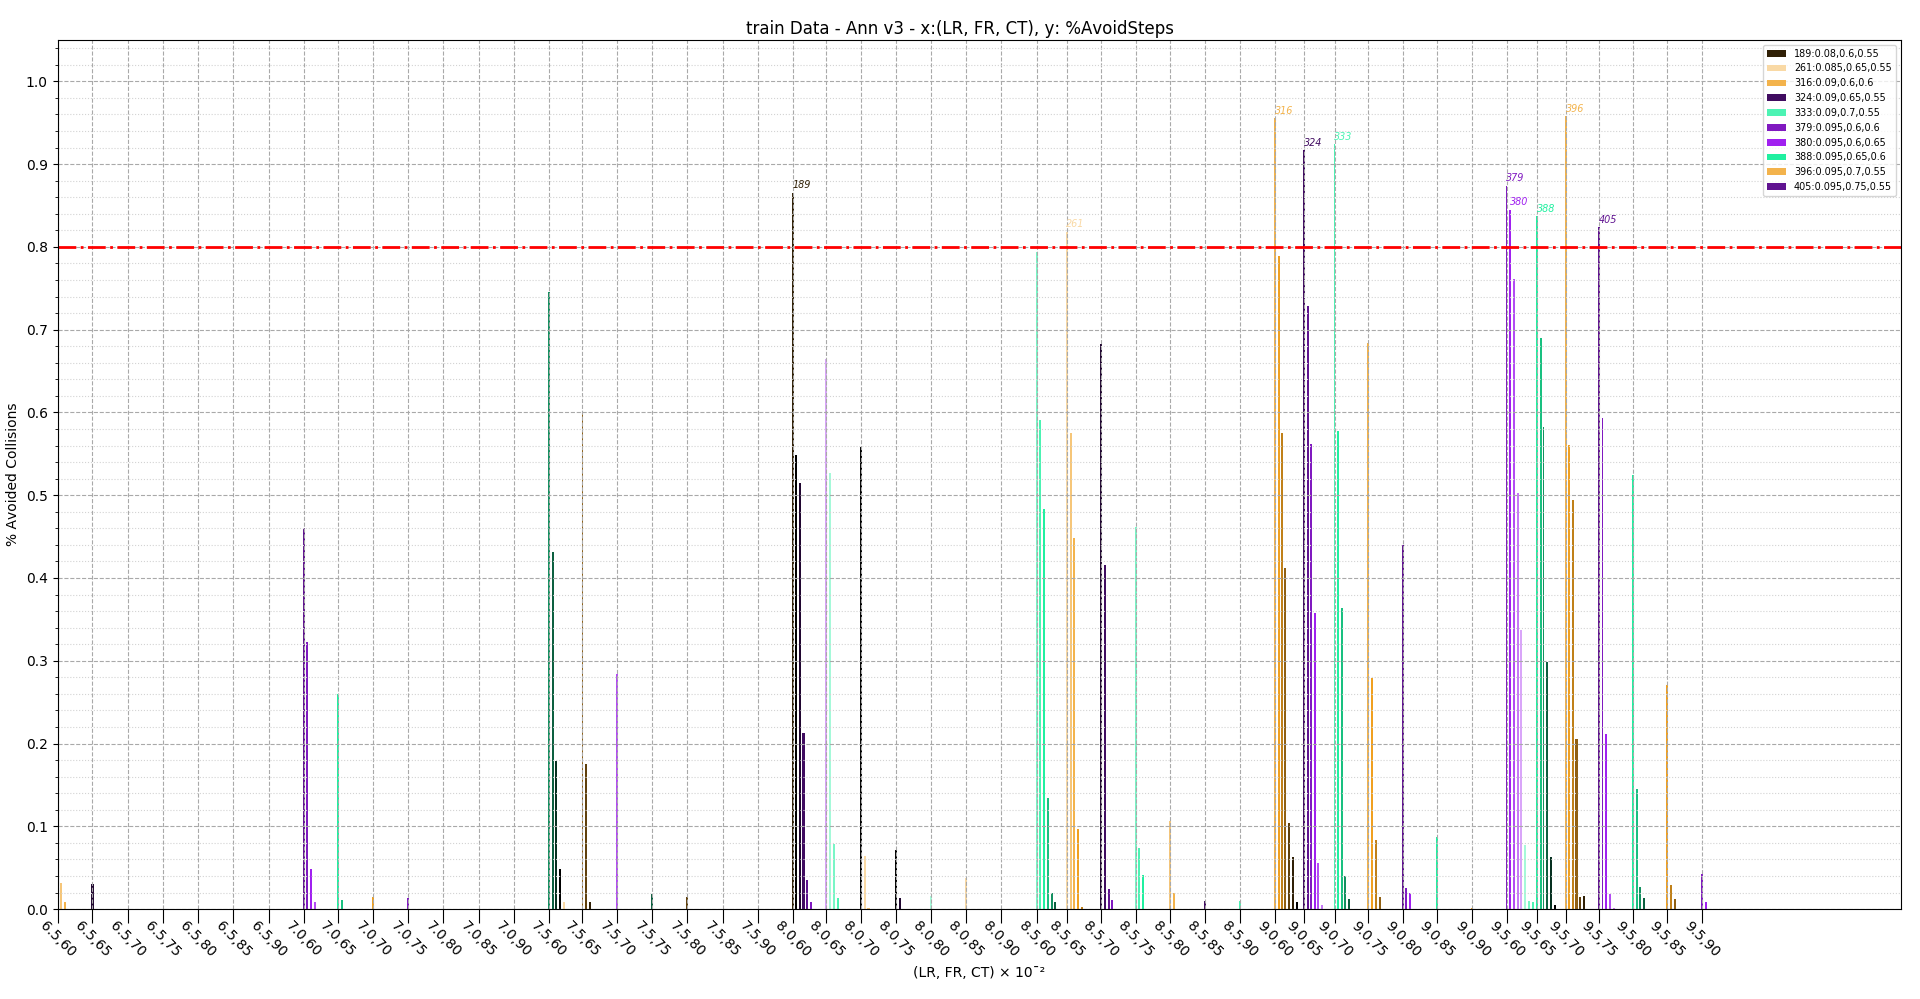
\includegraphics[scale=0.55,rotate=-90]{figures/train_annv3_2d.png}
    \caption{}
    \label{fig:TrainV3}
\end{figure}

\newpage
% \restoregeometry
\thispagestyle{empty}
% \newgeometry{top=5mm, bottom=10mm}

\begin{figure}[H]
    \centering
    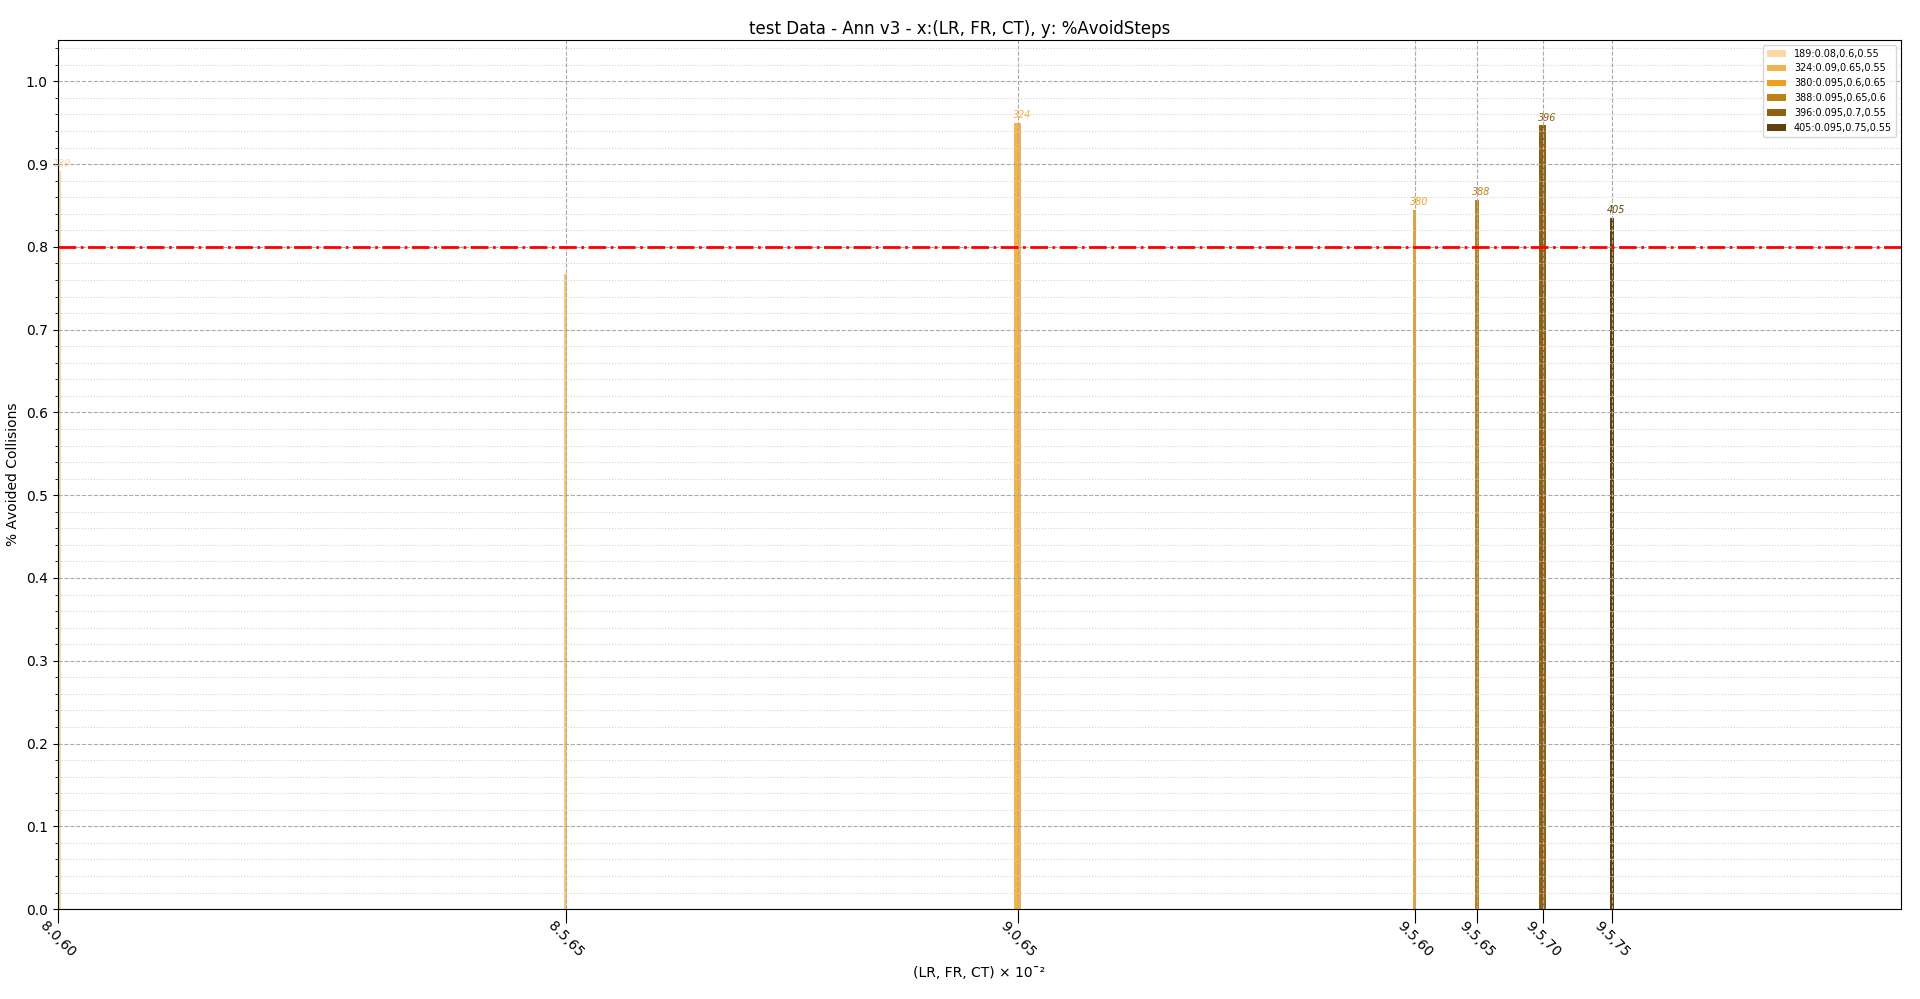
\includegraphics[scale=0.55,rotate=-90]{figures/test_annv3_2d.png}
    \caption{}
    \label{fig:TestV3}
\end{figure}

\newpage
% \restoregeometry
\thispagestyle{empty}
% \newgeometry{top=5mm, bottom=10mm}

\begin{figure}[H]
    \centering
    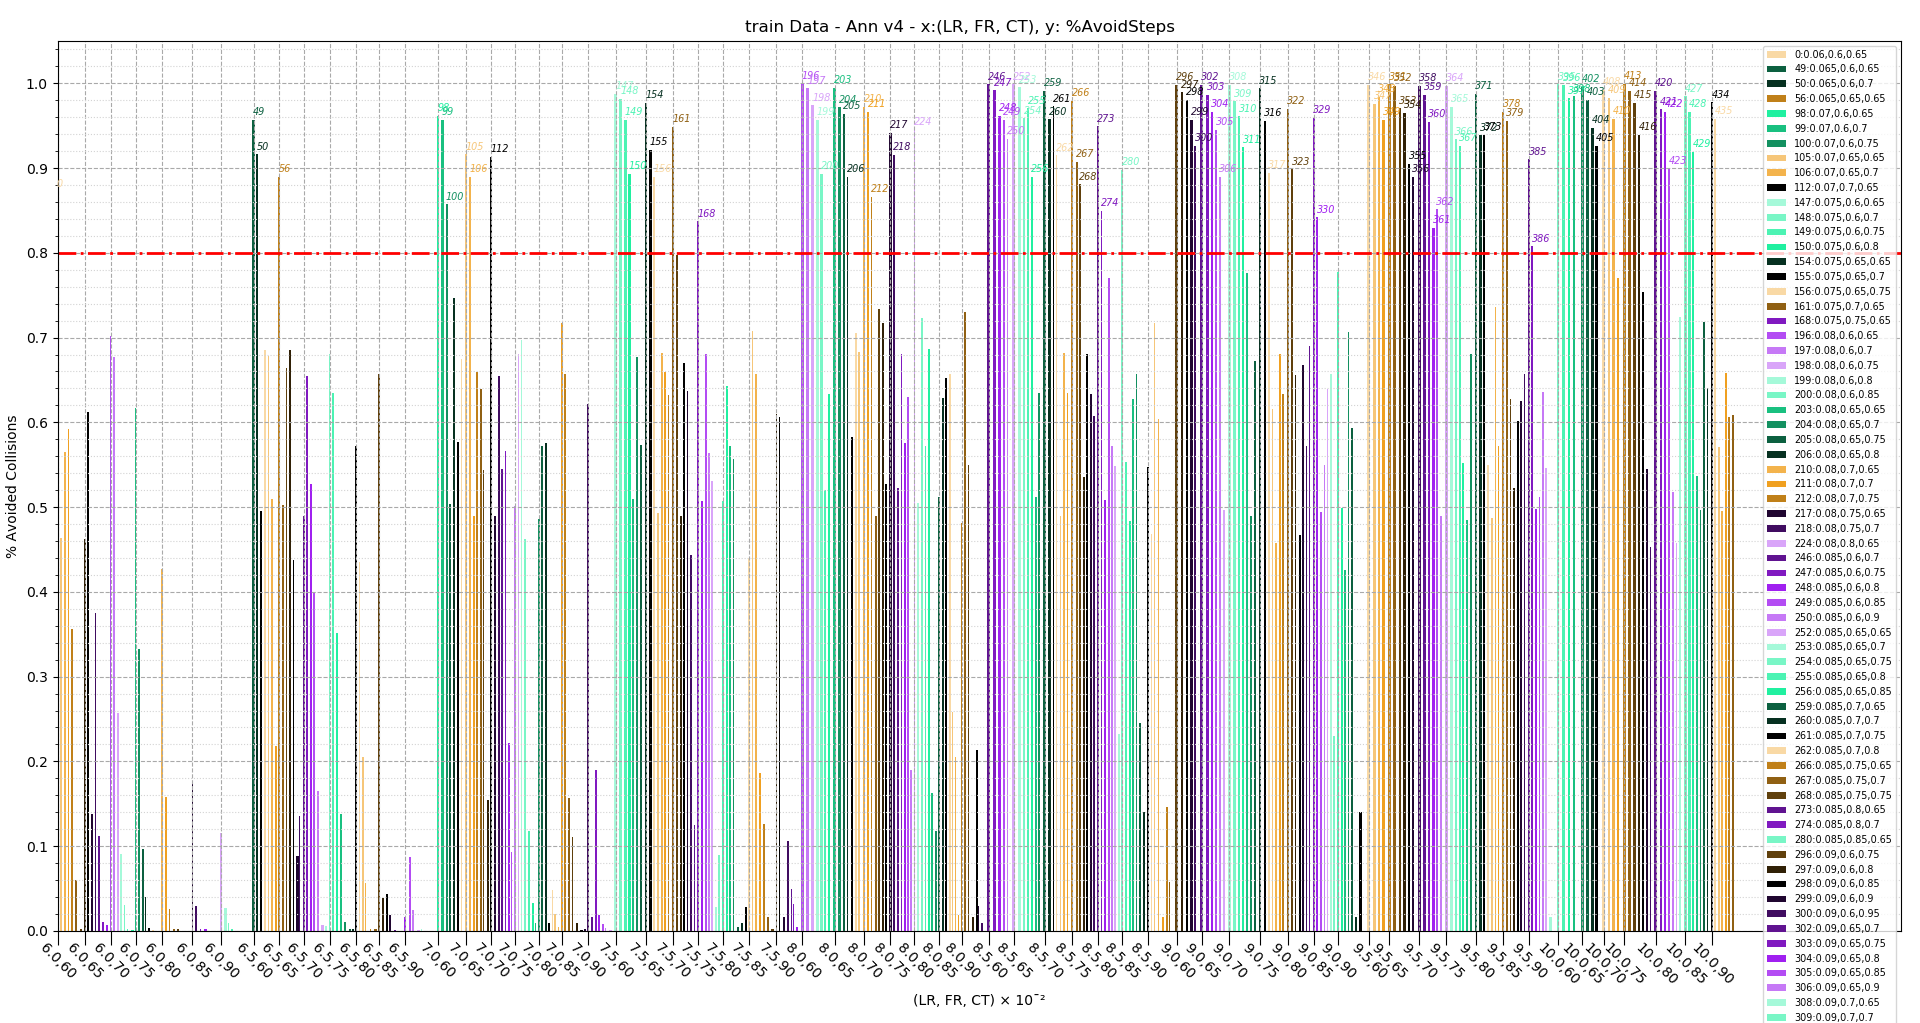
\includegraphics[scale=0.55,rotate=-90]{figures/train_annv4_2d.png}
    \caption{}
    \label{fig:TrainV4}
\end{figure}

\newpage
% \restoregeometry
\thispagestyle{empty}
% \newgeometry{top=5mm, bottom=10mm}

\begin{figure}[H]
    \centering
    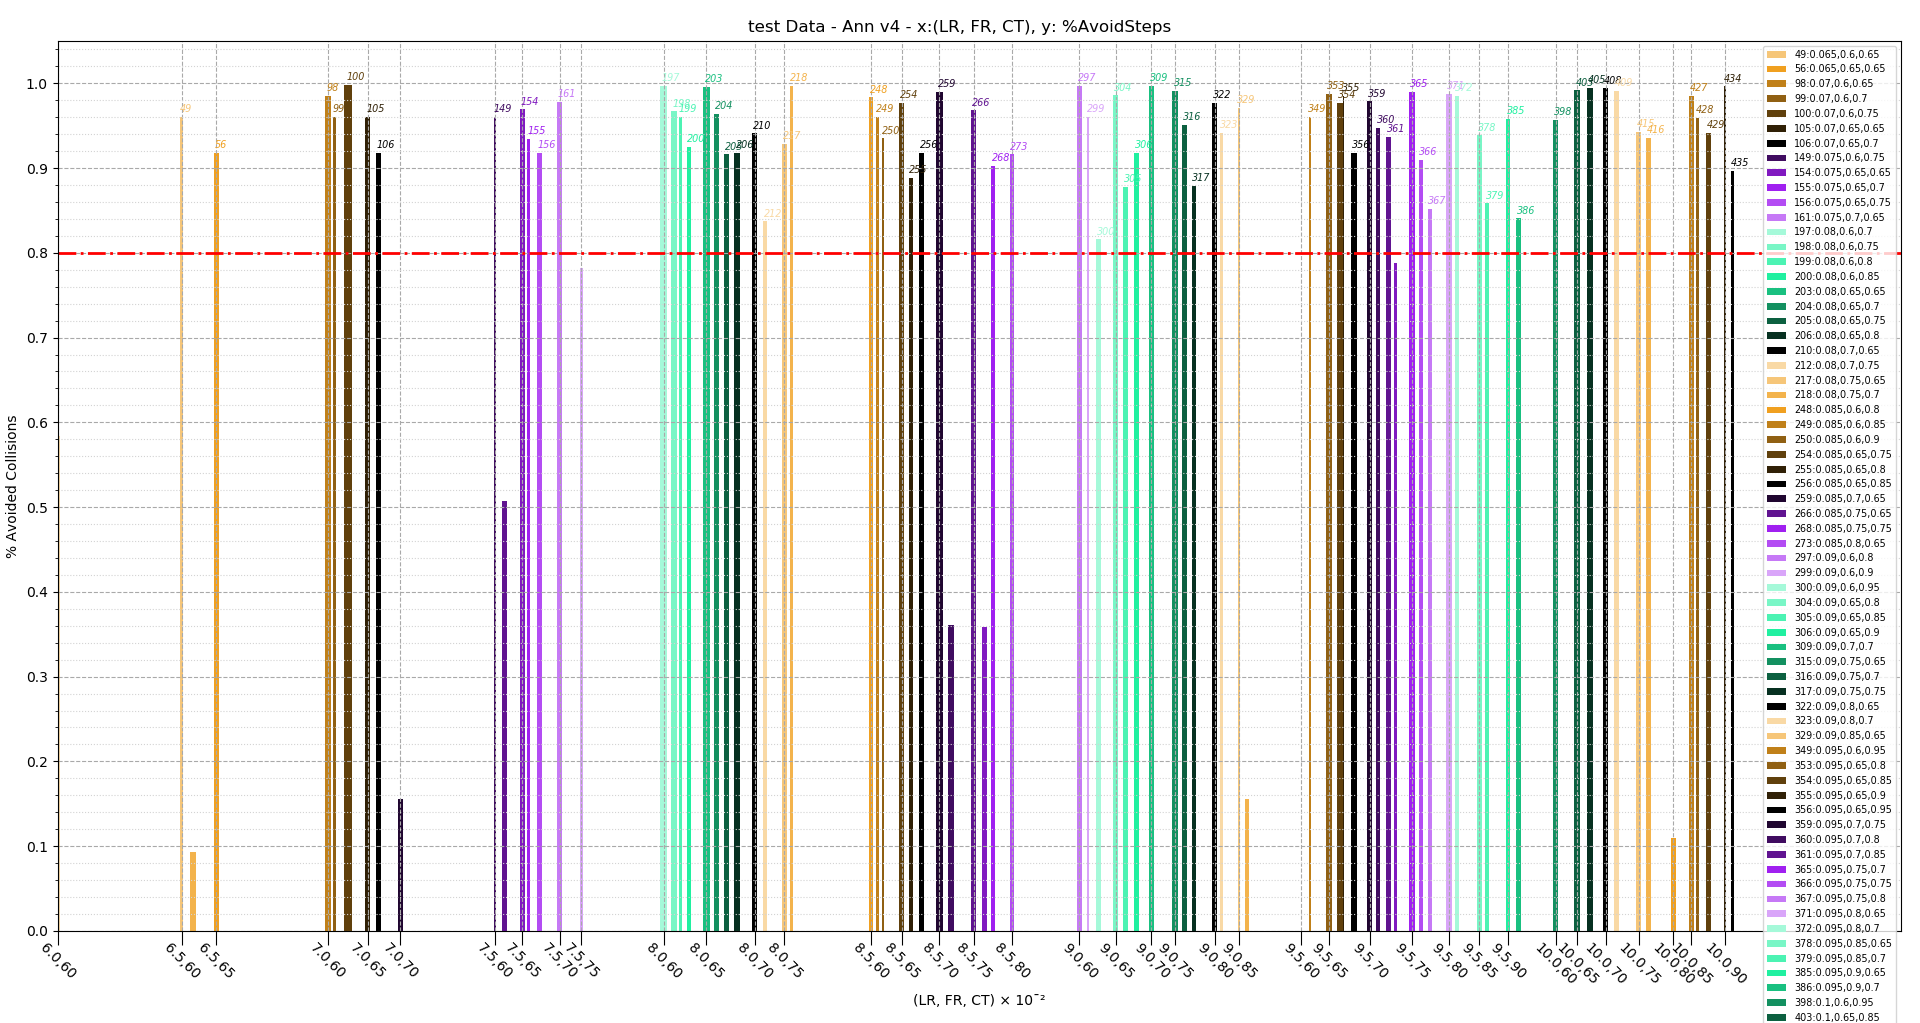
\includegraphics[scale=0.55,rotate=-90]{figures/test_annv4_2d.png}
    \caption{}
    \label{fig:TestV4}
\end{figure}

\newpage
\restoregeometry

% Esponi le problematiche che non si evincono dai dati

\paragraph{Addestramento e Test -- \texttt{dacv2}}\label{par:dacv2}\hfill

Durante gli studi preliminari per individuare una serie di esempi funzionanti attorno alla quale poi ricercare altre possibili configurazioni valide, si è notato un particolare "rapporto" tra i 3 parametri che guidano l'apprendimento: l'incremento di $\eta$ porta ad incrementare $\epsilon$.
Infatti, incrementare $\eta$ senza un adeguato aumento di $\epsilon$ conduce spesso il robot a conseguire un comportamento di tipo circolare. Questo è probabilmente riconducibile alla funzione di apprendimento adoperata che porta la rete ad essere facilmente affetta da \textit{overfitting}: anche per $\eta$ piccoli la rete degenera velocemente, portando il robot a non apprendere. Medesimo discorso vale per $\epsilon$: valori troppo bassi non permettono di compensare la natura saturante di $\eta$ ma, allo stesso tempo, valori eccessivamente elevati senza un adeguato contrasto di $\eta$ portano egualmente all'apprendimento di alcun meccanismo.

Il parametro $\tau_{Collision}$ si comporta in maniera abbastanza variabile rispetto agli altri due parametri ma costituisce un peso fondamentale che fa pendere l'ago della bilancia verso un stato di equilibrio o d'instabilità della rete. 

Questa serie di osservazioni ha portato ad esplorare solo una porzione dello spazio dei parametri per cui $\eta < \epsilon$. Quello che ci si aspettava dunque era di trovare, per ogni \texttt{learning rate} dell'intorno, almeno una coppia di $\epsilon$ e $\tau_{Collision}$ che producesse un modello valido. 

Com'è possibile vedere dai grafici \ref{fig:TrainV2} e \ref{fig:TestV2}, all'incrementare di $\eta$ le aree popolate da modelli "validi" sono in corrispondenza di zone in cui $\epsilon$ è via via leggermente più elevato. Questi poi si diradano quando $\epsilon$ diviene troppo elevato, a causa dell'eccessiva \textit{oscillazione della rete}. É inoltre interessante osservare come il numero di modelli "\textit{validi}" aumenta all'aumentare di $\eta$. Questo può essere riportato alle seguenti possibili motivazioni: 

\begin{enumerate}
    \item il tempo di addestramento (2h) per $\eta$ piccoli é troppo basso 
    \item $\epsilon$ per $\eta$ piccoli è troppo alta
    \item $\tau_{Collision}$ per $\eta$ piccoli è troppo alta
    \item la funzione di apprendimento utilizzata, in congiunzione al modello della rete neurale adoperata, raggiunge un effettivo equilibrio solo per valori elevati dei parametri
\end{enumerate} 

Una problematica dovuta alla presenza di questi parametri particolarmente sbilanciati è che, possedendo $\epsilon$ particolarmente grande, malgrado molti agenti apprendano velocemente il comportamento voluto, questi lo dimentichino anche altrettanto velocemente alla prima nuova collisione. Specialmente con un tempo di addestramento molto elevato, è avvenuto diverse volte che il robot imparasse ad evitare gli ostacoli modestamente ma il lavoro risultasse vanificato a causa di una collisione verso la conclusione del tempo di addestramento oppure perché l'agente si incastrasse in uno degli angoli concavi formati dagli ostacoli dell'arena.

Sebbene non sia stato esplorato completamente lo spazio dei parametri e dunque non siano state addestrate tutte le possibili configurazioni del modello, è evidente che se per valori così bassi di $\eta$ sono necessari valori particolarmente elevati di $\epsilon$ allora il restante spazio di ricerca, individuato \textit{incrementando} tali parametri, difficilmente può contenere ulteriori risultati significativi.
Altri scenari d'interesse esplorabili potrebbero essere quelli per cui $\eta < 0.035$ e $\epsilon < 0.65$, incrementando leggermente (verso il basso) il range dei valori di $\tau_{Collision}$ da esplorare.

Una caratteristica che si è notata in tutti gli agenti di \texttt{dacv2} che apprendono il comportamento desiderato di \textit{Obstacle-Avoidance} è quella di favorire uno specifico lato per evitare "correttamente"\footnote{Come ci aspetteremmo che l'agente eviti l'ostacolo.} gli ostacoli mentro sull'altro lato eseguono una piroetta prima di allontanarsi. Quest'ultimo comportamento "emergente" è, la maggior parte delle volte, la causa delle collisioni che il robot compie durante i suoi periodi di addestramento e test, sebbene questi abbia appreso la corretta associazione tra stimoli e risposte.

Questo comportamento "emergente", unito alla problematica precedentemente descritta, è una delle motivazioni per cui alcuni addestramenti producono un tipo di Falso Positivo particolarmente insidioso: comportamento circolare \textit{non su se stesso} (disegnando una serie di spirali) ma che dimostra egualmente \textit{Obstacle-Avoidance}. Questo particolare modello viene generato quando l'agente giunge vicino ad uno degli angoli concavi dell'arena con il lato che presenta il comportamento "emergente" rivolto verso gli ostacoli. Se questo genere di configurazione si presenta durante la fase di training, porta l'agente ad incastrarsi in un loop di piroette cercando di schivare ambedue gli ostacoli che compongono l'angolo; in fase di test ciò costringe invece l'agente a conseguire una traiettoria curvilinea e dunque presentare il comportamento "spiraliforme" sopra descritto.

A differenza degli altri Falsi Posiviti, dove la traiettoria circolare "in-place" è dovuta alla presenza di una serie di attivazioni costanti nel layer di Collisione, in questo caso il genere di traiettoria è provocata da una serie di \textit{attivazioni sporadiche}\footnote{Ovvero attivazioni non dovute ne ad una collisione ne alla presenza di ostacoli nelle vicinanze.} dei neuroni nel layer di Collisione che inducono il robot a sterzare quando non richiesto. Queste \textit{attivazioni sporadiche} posso essere ricondotte ad oscillazioni del modello della rete neurale appreso e dovute sia ai parametri di apprendimento particolarmente sbilanciati, sia all'interruzione dell'addestramento in una fase di apprendimento (modifica) dei pesi della rete. 

In entrambi i casi di Falsi Positivi, il loro comportamento può essere visto come una sorta di \textit{phantom pain} dell'agente e riportato al medesimo meccanismo: avendo troncato prematuramente l'apprendimento e dunque congelato il modello della rete neurale in una fase di disequilibrio, l'agente è attratto naturalmente ad eseguire più frequentemente l'ultima azione\footnote{Visto come pattern di attivazione dei neuroni nel layer di collisione} effettuata prima dell'arresto.

Per quanto riguarda in generale le prestazioni presentate nei grafici \ref{fig:TrainV2} e \ref{fig:TestV2}, è possibile osservare che le prestazioni migliori si ottengono per $\eta=0.065$ ma mostrando in generale valori inferiori rispetto agli score riportati in fase di addestramento. Al contrario, molti modelli che superano l'addestramento in maniera particolarmente brillante vengono identificati come Falsi Positivi durante i test, probabilmente a causa di una collisione prima della conclusione dell'addestramento.

\newpage

\paragraph{Addestramento e Test -- \textsc{dacv3}} \label{par:dacv3}\hfill

Per quanto riguarda il testing della versione \textit{dacv3} si è partiti prima di tutto ad effettuare un training e testing sfruttando gli stessi intervalli di parametri usati nella \textit{dacv2}. 

Purtroppo però, sia a livello qualitativo osservando il comportamento dell'agente che valutando quantitativamente i grafici, si è notato che tali configurazione fornivano risultati pessimi e in nessun caso riuscivano a portare l'agente ad apprendere. 
Si è quindi proceduto, come effettuato prima del training della \textit{dacv2}, ad una esplorazione empirica del possibile intervallo di valori dei parametri, il quale mostrasse una qualche forma di apprendimento di un comportamento corretto. A parità di \textit{forget rate} si è notato che l'agente cominciava a mostrare segni di apprendimento per valori di \textit{learning rate} maggiori di 0.65 e \textit{collision threshold} a partire da 0.55. 

È stato quindi effettuato un training in batch con intervallo di \textit{learning rate} tra 0.65 e 0.95 e \textit{collision threshold} tra 0.55 e 0.95. Successivamente sono stati selezionati i modelli che in fase di train presentavano una $\texttt{\%AvoidSteps} > 0.8$ per poi effettuare il test su essi.
Rispetto al modello \textit{dacv2} i modelli ottenuti, che presentano comportamenti di apprendimento significativi sono in numero minore, ma allo stesso tempo nessuno di quelli mostrati nel grafico relativo ai test (figura \ref{fig:TestV3}) è un falso positivo.

Osservando i grafici di train (figura \ref{fig:TrainV3}) si può notare che a parità di \textit{learning rate} e \textit{forget rate} aumentando la collision threshold la \texttt{\%AvoidSteps} tende a diminuire sensibilmente e i risultati migliori si ottengono per i valori tra 0.55 e 0.65. 
Sempre dal grafico \ref{fig:TrainV3} si evince che i valori più significativi si ottengono con valori di \textit{learning rate} a partire da 0.08 e si nota anche come all'aumentare del \textit{learning rate} la variazione della \textit{forget rate} e della \textit{collision-threshold} infici di meno sul valore di \texttt{\%AvoidSteps}.

Interessante risulta anche notare come sia in \ref{fig:TrainV3} che in \ref{fig:TestV3} per le coppie di valori [LR=0.09, FR=0.65] e [LR=0.95, FR=0.70] otteniamo dei valori di \texttt{\%AvoidSteps} molto simile.

Considerando che 0.55 è il valore minimo dell'intervallo di variazione della \textit{collision threshold} e considerando che alcuni risultati buoni sono stati ottenuti con tale valore, è stato interessante effettuare un'ulteriore run di training e test esplorando come intervallo il range [0.45,0.65]. Ciò è stato fatto con l'obiettivo di capire se al di sotto di 0.55 potevano essere presenti ulteriori valori interessanti. In questo caso si è scelto di concentrarsi su un intervallo di \textit{learning rate} contenenti i valori significativi ottenuti nella run mostrata nei grafici. Per la precisione $LR \in [0.085, 0.095]$. Mentre per quanto riguarda la FR è stato scelto il valore 0.6.
Ciò ha mostrato solo valori nulli di \texttt{\%AvoidSteps} al di sotto di una \textit{collision threshold} di 0.55.

Analizzando invece il comportamento a livello qualitativo, anche per quanto riguarda la versione \textit{dacv3} notiamo che l'agente apprende correttamente quando schivare gli ostacoli, ma effettuando schivate sempre verso destra, che nel caso in cui l'ostacolo si trovi da quella parte porta il robot ad effettuare una piroetta. Ciò è dovuto molto probabilmente alle stesse ragioni precedentemente esposte. 

Ricordando che la struttura della rete \textit{dacv3} è stata fatta sulla base della struttura descritta nel paper \cite{verschure1992distributed} e osservando il range di valori in cui abbiamo risultati migliori, si può notare che esso si avvicina ai valori dei parametri di apprendimento usati dagli autori del paper. Ciò può essere interpretato sia come una parziale conferma all'attendibilità dei valori riportati nel paper, sia come una corretta interpretazione da parte nostra del modello, nonostante l'assenza di alcuni elementi chiave. 

\newpage

\paragraph{Addestramento e Test -- \texttt{dacv4}}\label{par:dacv4}\hfill

Come già detto in fase di progettazione, \texttt{dacv4} nasce dal modello di \texttt{dacv2} al fine di comprendere come il comportamento e l'apprendimento di quest'ultima fosse influenzato dal numero di sensori, e dunque di neuroni, effettivamente utilizzati dall'agente. In tal senso questo modello si dimostra particolarmente interessante:

\begin{itemize}
    \item Da una parte il comportamento esterno dell'agente si è presentato non essere affatto dissimile da quello espresso utilizzando il modello di \texttt{dacv2}. Infatti, come per \texttt{dacv2}, il robot presenta i medesimi "pattern" di schivate: apprende "correttamente" a schivare l'ostacolo da un certo lato, ma per l'altro esegue una piroetta prima di allontanarsi. Questo lo porta a dimostrare anche le medesime problematiche presentate per \texttt{dacv2} e \texttt{dacv3}.
    
    \item Dall'altra, è qui risiede la fondamentale differenza dei due modelli, il quantitativo di modelli che risultano validi è cresciuto enormemente, attestandosi anche score particolarmente elevati. Malgrado non sia mostrato nei grafici, l'addestramento di \texttt{dacv4} nel medesimo spazio di parametri di \texttt{dacv2} ha prodotto solo qualche modello interessante per $\eta \ge 0.06$. Spostando l'addestramento verso parametri di apprendimento più elevati, $\eta \in [0.06, 0.1]$, il numero di modelli "validi" è incrementato esponenzialmente.
    
    Questo indica che il modello \texttt{dacv4} raggiunge l'equilibrio con valori di $\eta$ maggiori a parità dei medesimi spazi di ricerca per $\epsilon$ e $\tau$, portandosi leggermente più vicino ai valori di apprendimento riportati nel paper \cite{verschure1992distributed}. D'altro canto però tale risultato si pone come arma a doppio taglio in quanto è necessariamente sintomo di una maggiore probabilità di Falsi Positivi del secondo tipo (vedi \ref{par:dacv2}).
\end{itemize}

A differenza di \texttt{dacv2} le prestazioni in questo caso si dimostrano maggiormente constanti al variare dei parametri di apprendimento e decisamente più alte, sebbene alcuni dei modelli migliori come \texttt{100}, \texttt{197} e \texttt{297} risultano essere dei Falsi Positivi del secondo tipo.  




\section{Conclusioni}

Alla luce dei risultati ottenuti possiamo dire che tutti i modelli di reti imparano a schivare gli ostacoli più o meno bene. 

Osservando i risultati dei comportamenti di \textit{Collision-Avoidance} ottenuti da \texttt{dacv2} in relazione alle sue controparti \texttt{dacv3} e specialmente \texttt{dacv4}, possiamo constatare che l'utilizzo dei bumper e sensori di prossimità posteriori influenzi negativamente sull'apprendimento del comportamento da parte dell'agente. 

Dai grafici risultanti dai dati ottenuti durante gli esami di addestramento e test, presentati nella precedente sezione, si può notare come la presenza di più neuroni nel layer di Collisione nei modelli \texttt{dacv2} e \texttt{dacv4} permetta però all'agente di apprendere decisamente meglio il comportamento al variare di uno dei parametri. Mentre per quanto riguarda \texttt{dacv3} essa è in grado di apprendere solo per un ristretto intorno di parametri di apprendimento $\tau \ge 0.09$.

Considerando il problema presentato da tutte tre i modelli, di apprendere correttamente a schivare gli ostacoli da un solo lato mentre dall'altro esegue una piroetta prima di allontanarsi, oltre ai possibili accorgimenti per far fronte alle problematiche discusse nella sezione di test, una prima soluzione potrebbe essere individuata scegliendo casualmente il lato di inversione della marcia in caso di parità. 

Alternativamente un'esplorazione interessante potrebbe consistere nell'integrazione della \textit{Fototassi} al comportamento di \textit{Collision-Avoidance}, la quale potrebbe permettere all'agente di apprendere la \textit{Collision-Avoidance} con maggiore efficienza in quanto vi è un obiettivo preciso da raggiungere, piuttosto che vagare per l'arena senza una meta. Ciò \textit{potrebbe} anche risolvere quei casi in cui l'agente si incastra negli angoli concavi dell'arena, producendo il comportamento con moto a spirale/circolare, oppure evitare che l'agente carichi semplicemente un ostacolo all'inizio dell'addestramento, evitando in entrambi casi che la rete vada facilmente in \textit{overfitting}.

Un'altra possibile soluzione per risolvere il problema presentato potrebbe essere quello di effettuare ulteriori addestramenti in arene differenti che permettano di bilanciare meglio le risposte agli stimoli e quindi offrire la possibilità all'agente di generalizzare più correttamente il proprio comportamento.

Potrebbe essere inoltre utile anche esplorare a livello temporale quale sia in media il tempo ottimale di addestramento, anche se questo risulterebbe particolarmente legato al modello di arena utilizzato.

Inoltre sarebbe interessante determinare la conclusione dell'addestramento sulla base di una funzione di \textit{fitness} che permetta di descrivere la bontà del comportamento appreso in maniera incrementale. In tal modo si terminerà l'addestramento qualora tale \textit{fitness value} superi una determinata soglia, evitando di troncare la simulazione nel corso di una fase si instabilità della rete neurale.
\hfill\break
Detto ciò passiamo a fare un'analisi ed un confronto quantitativo dei dati ottenuti dai tre modelli. 

In questo caso rispetto ai grafici precedenti, in cui veniva utilizzata la sola \textit{\%AvoidanceStep} come  metrica di confronto dei modelli addestrati, prendiamo in considerazione anche le deviazioni standard sugli assi x e z. Tale scelta nasce a posteriori dalla necessità di voler cercare di tenere in considerazione la presenza di possibili Falsi Positivi nei test. Per tale motivo il confronto tenderà a preferire quei modelli che permettono all'agente robotico di esplorare maggiormente l'arena. Si è quindi proceduto prendendo per prima cosa tutti i valori di test dei 3 modelli. Essi sono stati poi filtrati in modo da eliminare tutti i risultati che presentavano $\texttt{std(x)} < 0.2 \quad\wedge\quad \texttt{std(z)} < 0.2$. Una volta fatto ciò è stata definita una metrica di ranking che permettesse di ordinare i modelli, tenendo in considerazione \texttt{\%AvoidStep}, deviazione standard media sugli assi e deviazione standard delle deviazioni standard sugli assi. 

$$\overline{\texttt{STD}}_i = mean(\{\texttt{std(x)}_i, \texttt{std(z)}_i\})$$

$$\texttt{std(x, z)}_i = std(\{\texttt{std(x)}_i, \texttt{std(z)}_i\})$$

$$rank_i = \frac{\overline{\texttt{STD}}_i \cdot 0.35 - \texttt{std(x, z)}_i \cdot 0.05 + \texttt{\%AvoidSteps}_i \cdot 0.6}{0.35 + 0.05 + 0.6}$$

\hfill\break

Come si può notare dalla formula si è fatto ricorso anche all'uso della media pesata. Essa permette di prediligere quei modelli che offrono score di "avoidance" elevati e variazioni significative su entrambi gli assi, penalizzando quelli che presentano variazioni soltanto di un asse. 

Mostriamo ora una tabella contenente i primi 15 modelli confrontati con la metrica sopracitata.

\begin{table}[H]
    \centering
    \begin{tabular}{|c|c|c|c|c|c|c|c|}
        \hline
        i	&   v	&	$\eta$,$\epsilon$,$\tau$ &   mAvoidSteps	& \%AvoidSteps & std(x) & std(z) & rank \\
        \hline
        157	    &   2	    &	0.05,0.65,0.8     &   11.71	&   0.9388	&   0.6797	&   0.6075	& 1 \\
        361	    &   4	    &	0.095,0.7,0.85 	&   10.82	&   0.9370	&   0.6602	&   0.6128	& 0.99840 \\
        409	    &   4	    &	0.1,0.7,0.8       &   9.14	&   0.9912	&   0.6376	&   0.4267	& 0.99380 \\
        427	    &   4	    &	0.1,0.85,0.65   	&   10.03	&   0.9852	&   0.5115	&   0.5391	& 0.99302 \\
        385	    &   4	    &	0.095,0.9,0.65   	&   14.86	&   0.9585	&   0.6765	&   0.4883	& 0.99298 \\
        353	    &   4	    &	0.095,0.65,0.8    &   7.79	&   0.9872	&   0.5094	&   0.4924	& 0.98906 \\
        155	    &   4	    &	0.075,0.65,0.7    &   20.49	&   0.9349	&   0.7576	&   0.4576	& 0.98843 \\
        337	    &   2	    &	0.065,0.9,0.7     &   9.56	&   0.9666	&   0.4938	&   0.5562	& 0.98623 \\
        372	    &   4	    &	0.095,0.8,0.7     &   15.73	&   0.9854	&   0.5912	&   0.4099	& 0.98608 \\
        324	    &   3	    &	0.09,0.65,0.55   	&   7.57	&   0.9499	&   0.5415	&   0.5493	& 0.98538 \\
        403	    &   4	    &	0.1,0.65,0.85   	&   7.07	&   0.9918	&   0.5341	&   0.4197	& 0.98454 \\
        217	    &   4	    &	0.08,0.75,0.65   	&   13.38	&   0.9284	&   0.5802	&   0.5690	& 0.98384 \\
        396	    &   3	    &	0.095,0.7,0.55   	&   7.74	&   0.9469	&   0.5420	&   0.5418	& 0.98380 \\
        175	    &   2	    &	0.05,0.8,0.65   	&   10.62	&   0.9291	&   0.5315	&   0.6139	& 0.98268 \\
        \hline
    \end{tabular}
    \caption{Top 15 trained models among the 3 different type.}
    \label{tab:ranks}
\end{table}

Consci che un confronto più rigoroso richieda ulteriori test e training con ulteriori parametri differenti e utilizzando arene differenti. Siamo nel complesso abbastanza soddisfatti dei risultati ottenuti. 
Il progetto ci ha permesso di sperimentare per la prima volta un utilizzo in pratica delle reti neurali e renderci conto di come esse, nonostante a prima vista possano sembrare semplici, spesso sorprendono mostrando comportamenti emergenti inaspettati a cui è complicato dare spiegazioni semplici al primo colpo.  

\nocite{*}
\addcontentsline{toc}{section}{Riferimenti bibliografici}
% Elencare i riferimenti bibliografici citati nel testo. 
\bibliography{References.bib}
\bibliographystyle{plain}

%----------------------------------------------------------------------------------------

\end{document}
